\chapter{Design}

In this chapter, we lay out the requirements for our implementation of Wasm containers in Apache OpenWhisk. Then we describe and discuss our implementation and the trade-offs involved.

\section{Requirements}

\subsection{Apache OpenWhisk}

In order to understand the requirements for our Wasm-flavored OpenWhisk, we need to understand the design of OpenWhisk itself first.

\begin{figure}
    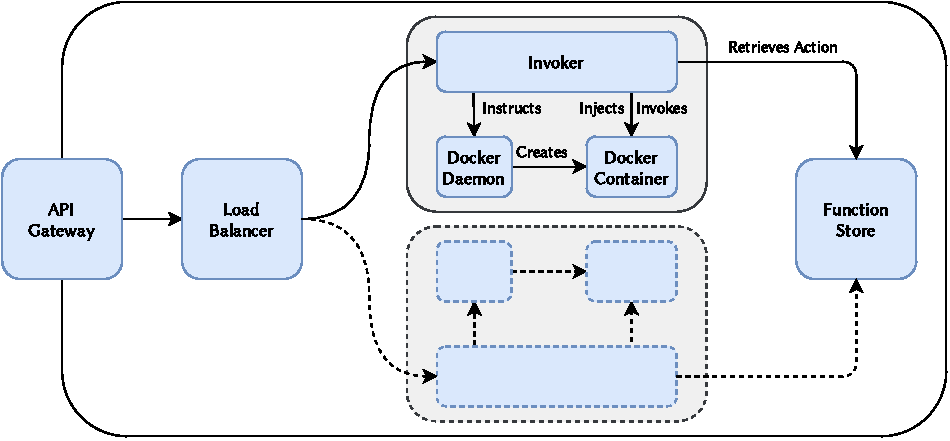
\includegraphics{figures/OpenWhiskActionInvocationFlow.pdf}
    \caption{Action invocation flow in Apache OpenWhisk based on the source code and documentation \cite{OpenWhiskSystemDesign}. Potentially many Invokers can exist in this setup.}
    \label{fig:openwhisk-action-invocation-flow}
\end{figure}

Figure \ref{fig:openwhisk-action-invocation-flow} sketches the design of OpenWhisk. Users interact with it through its API Gateway, which consists of \inl{nginx}, mostly for SSL termination, and the \inl{Controller}, which implements the main logic. It handles the creation of actions, OpenWhisk's name for serverless functions, authentication and authorization as well as invoking the action.
In the latter case, the controller uses its load balancer to determine which Invoker should handle the request, and publishes the request to an Apache Kafka queue, which the invoker is subscribed to. The controller and its load balancing take a central role in OpenWhisk, but in our figure it is represented by the API Gateway and the Load Balancer only, simply because we will not be modifying this part.
Our focus is on the Invoker. It is the part of OpenWhisk responsible for \emph{invoking} the action. A number of steps are involved in that process \cite{OpenWhiskSystemDesign}.

\begin{enumerate}
    \item It retrieves the action's code and execution permissions from an Apache CouchDB database, where the Controller stored it during action creation. 
    \item It instructs the local Docker daemon to start a new container, based on the runtime that the action needs to execute. This would be a \inl{openwhisk/action-nodejs-v10} image for JavaScript actions but could also be a generic black-box image (\inl{openwhisk/dockerskeleton}), that can execute any binary, such as one written in Rust or C.
    \item Finally, it injects the action's code into the container, invokes it with the given parameters and returns the result \cite{OpenWhiskSystemDesign}.
\end{enumerate}

Because OpenWhisk supports many runtimes and even the mentioned black-box image, it needs a common protocol to communicate with all of them. The just-described step 3 is the gist of that protocol. Each runtime needs to implement three endpoints. The \inl{/start} endpoint creates a new container and returns its address. The following requests to the \inl{/init} endpoint are then sent to that address, where the container receives the code and takes whatever steps necessary to make the action ready for execution. Thus, over a containers life cycle, this endpoint is called exactly once. Once initialized, the \inl{/run} endpoint can be called multiple times to execute the action \cite{OpenWhiskSystemDesign}.

That implies that the container isn't destroyed immediately after it has been invoked once. Indeed, OpenWhisk uses various optimizations of the described flow, in order to improve the system's performance. Among those are pre-warming containers or keeping the container running for some time after it has been invoked, before it is removed.
We will explore those optimizations in more depth later, to compare them to the optimizations in our Wasm runtime to better see where they coincide and differ \cite{OpenWhiskSystemDesign}.

\subsection{OpenWhisk on Kubernetes}

OpenWhisk can be deployed on a Kubernetes cluster, a container orchestration tool for automating deployment and scaling of containers \cite{Kub2021}. OpenWhisk has a \inl{ContainerFactoryProvider} service provider interface (SPI), which represents the underlying container management platform. It provides two implementations of that SPI \cite{OWKub2020}.

\begin{enumerate}
    \item The \inl{DockerContainerFactory} implements the architecture shown above, except that most components of OpenWhisk run in separate Kubernetes pods. In non-Kubernetes deployments, they usually run in separate Docker containers. The crucial part of this deployment is, that the Invoker runs in a single pod (potentially on multiple worker nodes), and also spawns all of the actions in docker containers inside that pod. Thus container management latency is rather small, but does not take advantage of Kubernetes' scaling mechanisms.
    \item The \inl{KubernetesContainerFactory} interfaces with the Kubernetes API to create and schedule actions in containers -- in turn contained in pods -- to run on different Kubernetes worker nodes. This trades higher container management latency for access to Kubernetes' scaling mechanisms.
\end{enumerate}

\subsection{Executing WebAssembly with OpenWhisk}

To execute Wasm modules in OpenWhisk, we have two similar options with similar trade-offs.

\begin{enumerate}
    \item Using one of a number of WebAssembly runtimes that are currently being developed and are in various stages of maturity. We would need to embed one of these runtimes in a program of our own that provides a similar interface as Docker. This WebAssembly container runtime would then be able to replace the Docker daemon in the architecture presented above, and run Wasm modules instead of Docker images. Since this program would sit in-between OpenWhisk and the Wasm runtime, we would have precise control over the management of the modules, i.e. whether the Wasm module is just-in-time compiled, interpreted or compiled to native code ahead-of-time; the caching layer that keeps initialized modules ready for fast execution; or the configuration of the system interface with which Wasm modules can interact with the underlying operating system.
    \item The second option is to use Kubernetes as the management system for our Wasm modules. Kubernetes is generic over the underlying container runtimes, and as such it runs on \inl{containerd}, \inl{CRI-O} and Docker \cite{Kub2021}. However, it is also possible to let Kubernetes pods run on other runtimes by implementing the \inl{kubelet} API. The \inl{krustlet} project provides a \inl{kubelet} implementation that can execute Wasm workloads \cite{Krustlet2021}. With that, we can now instruct Kubernetes to run Wasm modules for us, instead of the typical Docker container.
\end{enumerate}

We will explore those two options in more detail and discuss which may be a better fit for our requirements.

\subsection{Krustlet: The WebAssembly Kubelet}

As a \inl{kubelet}, \inl{krustlet} runs on Kubernetes worker nodes and accepts workloads of the \inl{wasm32-wasi} architecture. Just like a regular kubelet, krustlet will then pull the Wasm module from an OCI registry and run it. We could thus schedule our Wasm workloads from an Invoker, similar to how the \inl{KubernetesContainerFactory} implementation schedules actions in Docker containers. However, this execution model is also different from the OpenWhisk model in some ways.

\begin{itemize}
    \item In OpenWhisk there is a split between runtime environment, provided through the Docker image, and the code that is stored in a database, retrieved from there and injected into the container. Krustlet expects the Wasm module to be the equivalent of the container, but with the code baked in. Thus no injection is necessary. This makes it slightly harder to integrate with the current OpenWhisk model, since the Wasm module doesn't need to be stored in the database, but rather in the OCI registry. That registry would need to be part of the Kubernetes cluster, since the images are not generic runtime environments, but the Wasm modules uploaded to OpenWhisk by the users. We can assume, that the latency introduced by retrieving the image from the registry is offset by not having to retrieve the code from the database, so both solutions should perform the same in that regard.
    \item Since there is no split anymore, every Wasm module needs to implement the OpenWhisk runtime protocol itself, instead of being able to rely on the runtime. In practice, this means implementing the \inl{/init} and \inl{/run} endpoints, where the former would no longer do anything useful, since there is no code to inject. Because network support in WASI is still under active development, the alternative is to implement a \inl{wasmcloud-actor}, which essentially provides capabilities such as networking to Wasm modules \cite{WC2021}. The function can then be run by calling the \inl{/run} endpoint. Just like containers in OpenWhisk keep running for some time after having been called once, the module would also continue to listen for more requests to avoid the cold-start.
\end{itemize}

While this approach has its merits, we believe that there would be higher friction for implementing it in OpenWhisk, than writing our own layer to Wasm runtimes. It provides more control over optimizing the cold-start latency as well as the execution performance, which are our main priorities.

\subsection{OpenWhisk Modifications}

% Figure Planned modifications which is directly comparable to aboves figure

\begin{figure}
    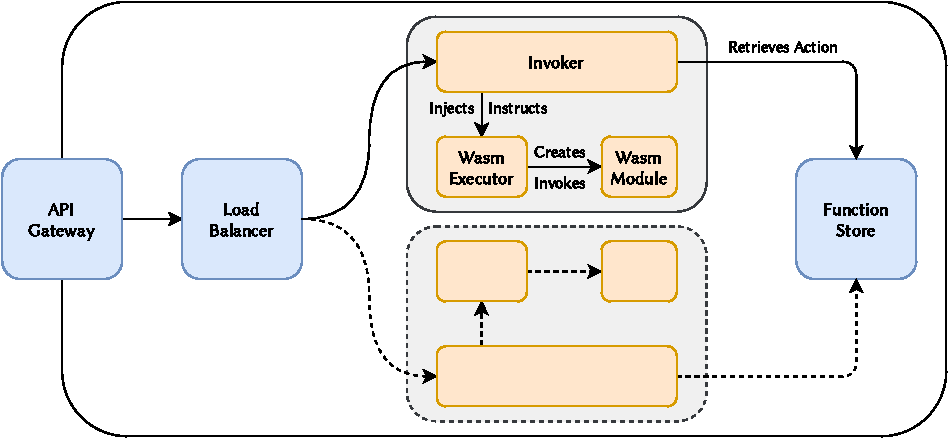
\includegraphics{figures/WasmOpenWhiskActionInvocationFlow.pdf}
    \caption{Invocation flow of a Wasm action in our modified Apache OpenWhisk.}
    \label{fig:wasm-openwhisk-action-invocation-flow}
\end{figure}

In this described invocation flow, we need to hook into OpenWhisk's invoker to enable its communication with the Wasm runtime we will implement, instead of the Docker daemon. Fortunately, the Invoker is already well-separated from the concrete containerization technology through a Service Provider Interface (SPI). OpenWhisk already supports Docker, but also Kubernetes as the container management system, such that the SPI was a logical addition. We implement a \inl{WasmContainer} that extends OpenWhisk's \inl{Container} abstraction, which already handles container communication, such as calling the \inl{/init} and \inl{/run} endpoints.

% Figure that shows a zoomed-in version of the invoker and its SPIs (as well as the Wasm runtime?) - Help better understand OW's design and what we added

In OpenWhisk's Docker container implementation, OpenWhisk only uses the Docker daemon to create a container, but then communicates with the container directly. In our implementation, every request is proxied through the \inl{WasmRuntime}. The advantage is, that not every Wasm module needs to implement the OpenWhisk protocol, which requires an HTTP server; increasing both the module's size and its runtime overhead. That presupposes, that the \inl{WasmRuntime} can handle a potentially large amount of requests.

% Need to decide whether OW handles containers life cycle or if runtime takes that responsibility

The runtime also needs to be fast in general, in order to aid in alleviating the cold start problem. That includes efficient handling of receiving the module's code from OpenWhisk, instantiating it and setting up the underlying Wasm executor. A general requirement for a useful Wasm runtime would also be its ability to run on different instruction set architectures.

In summary, the requirements for our runtime are

\begin{enumerate}
    \item It needs to be fast to alleviate the cold-start problem.
    \item It needs to run on devices with potentially different instruction set architectures.
    \item It needs to be able to efficiently handle a large amount of I/O concurrently, due to all requests being proxied through
\end{enumerate}

\section{Implementation}

To implement these requirements in Apache OpenWhisk we will take the following steps. The current Docker-based invoker will be replaced, to forward all the incoming requests to our new Wasm runtime.

The Wasm runtime will be written from scratch in the Rust programming language. There are a number of reasons for this choice.

\begin{itemize}
  \item It is a compiled language with performance close to that of C.
  \item It uses LLVM in the backend so that it can be compiled for almost any architecture.
  \item It allows for \quot{fearless concurrency}, since the compiler can detect data races at compile time.
  \item It has good support for asynchronous I/O, so it should be able to efficiently handle a large amount of concurrent requests.
  \item 3 out of the 4 Wasm executors investigated here are written in Rust, so embedding them is efficient and well documented.
\end{itemize}

The runtime consists of a web server that can take requests from the invoker asynchronously and concurrently. Because OpenWhisk doesn't communicate with the Wasm modules directly, but through the runtime, the \inl{/start} endpoint simply returns the runtimes own network address. This endpoint also returns an identifier for the container, so that OpenWhisk can handle its life cycle, i.e. the above-mentioned mechanism of keeping it warm for some time, for a faster subsequent invocation. There is a chance that this mechanism may not be necessary for Wasm modules, as they are much more lightweight in their instantiation. We will come back to this question later in our optimization discussion.

The entry point into our runtime will be through HTTP endpoints. In order for our runtime to handle requests concurrently, we use Rust's \inl{async} features. We will not make use of any advanced HTTP features, so the choice of the web framework doesn't matter too much. We use \inl{tide} \cite{Turon2021}, an asynchronous by-default web framework ideal for prototyping. It builds on top of \inl{async-std}, the asynchronous version of the Rust standard library.
Rust's async model works with \inl{Futures} -- also known as Promises in JavaScript -- which represent values that have not yet been computed. Contrary to \inl{Promises} however, Rust's \inl{Futures} are lazy: They do nothing unless actively polled. This task falls to \inl{async} runtimes, of which \inl{async-std} provides one. In \inl{async-std} the unit of execution is a \inl{Task}, which is similar to a \inl{Thread}, except it is driven to completion by the user space runtime instead of the OS. Many of those tasks are executed on the same thread, and by default, a \inl{Thread} per logical CPU core is spawned. Thus we have $M \cdot N$ tasks in total, where $M$ is the number of tasks per thread and $N$ the number of logical CPU cores.
From that, a second distinction is implied. A \inl{Task} should not do a blocking or long-running operation, like reading from a file via the standard library's \inl{std::fs::read_to_string}. Instead, it should use the \inl{async} version of that method, from \inl{async-std}, which does not block the thread. Otherwise, all other $M - 1$ tasks, which are executed on the same thread, will also be blocked, even though they may be able to make progress. Note that, we could still process $N$ requests concurrently, even if tasks block, but that doesn't scale well enough. This is why async functions are also called cooperative routines (coroutines). When they need to wait for the OS to finish a task, they \emph{yield} to another routine, which can then continue actual work.

That becomes relevant for us, when we execute WebAssembly modules. Taking the module, setting up the Wasm runtime and executing it, is a long-running computation -- and one that could block as well. This would in turn block the thread we are currently running on, which means, only $N$ Wasm modules can be executed concurrently. This is not an issue for computationally-intensive workloads, where no more work can be done concurrently, than the CPU has logical cores. However, for I/O-bound workloads, such as requests over the network, this can quickly become a bottleneck. Since one of the appealing offerings of serverless frameworks is their elasticity, we clearly need a way to handle many more requests, even if they block.
To let other coroutines on the same thread make progress, while one executes the module, we can push the entire execution onto a thread pool. The coroutine then has the simple job to asynchronously wait for that execution to finish and collect the result. That allows the other coroutines to process more requests in the meantime.

To test the theory, whether the thread pool model is able to handle more requests, we run two short experiments.

\begin{enumerate}
    \item Compute-bound: Calculating a large prime number.
    % \item Filesystem-I/O-bound: Reading a 30 MB file from disk.
    \item Network-I/O-bound: Making a long-running (1 second) HTTP request.
\end{enumerate}

Our test machine has 8 logical CPU cores, resulting in 8 threads being started for the async-std runtime. We thus send 16 concurrent requests to be able to see the potential blocking in the result. The first experiment showed no difference in the total execution time between the default and thread pool model. As we would expect, in the default model the compute-bound task finishes the first 8 requests, before starting the second set. The execution in a thread pool executes all 16 requests concurrently, but each took roughly twice as long, resulting in no significant difference between the total execution time. The default model operates more along the first-come, first-serve principle, where an early request will also get a response more quickly. In this simplified example, where all workloads are compute-bound, this may be preferable.

\begin{figure}
    \begin{center}
        %% Creator: Matplotlib, PGF backend
%%
%% To include the figure in your LaTeX document, write
%%   \input{<filename>.pgf}
%%
%% Make sure the required packages are loaded in your preamble
%%   \usepackage{pgf}
%%
%% and, on pdftex
%%   \usepackage[utf8]{inputenc}\DeclareUnicodeCharacter{2212}{-}
%%
%% or, on luatex and xetex
%%   \usepackage{unicode-math}
%%
%% Figures using additional raster images can only be included by \input if
%% they are in the same directory as the main LaTeX file. For loading figures
%% from other directories you can use the `import` package
%%   \usepackage{import}
%%
%% and then include the figures with
%%   \import{<path to file>}{<filename>.pgf}
%%
%% Matplotlib used the following preamble
%%   \usepackage{fontspec}
%%
\begingroup%
\makeatletter%
\begin{pgfpicture}%
\pgfpathrectangle{\pgfpointorigin}{\pgfqpoint{5.809079in}{4.647263in}}%
\pgfusepath{use as bounding box, clip}%
\begin{pgfscope}%
\pgfsetbuttcap%
\pgfsetmiterjoin%
\definecolor{currentfill}{rgb}{1.000000,1.000000,1.000000}%
\pgfsetfillcolor{currentfill}%
\pgfsetlinewidth{0.000000pt}%
\definecolor{currentstroke}{rgb}{1.000000,1.000000,1.000000}%
\pgfsetstrokecolor{currentstroke}%
\pgfsetdash{}{0pt}%
\pgfpathmoveto{\pgfqpoint{0.000000in}{0.000000in}}%
\pgfpathlineto{\pgfqpoint{5.809079in}{0.000000in}}%
\pgfpathlineto{\pgfqpoint{5.809079in}{4.647263in}}%
\pgfpathlineto{\pgfqpoint{0.000000in}{4.647263in}}%
\pgfpathclose%
\pgfusepath{fill}%
\end{pgfscope}%
\begin{pgfscope}%
\pgfsetbuttcap%
\pgfsetmiterjoin%
\definecolor{currentfill}{rgb}{0.917647,0.917647,0.949020}%
\pgfsetfillcolor{currentfill}%
\pgfsetlinewidth{0.000000pt}%
\definecolor{currentstroke}{rgb}{0.000000,0.000000,0.000000}%
\pgfsetstrokecolor{currentstroke}%
\pgfsetstrokeopacity{0.000000}%
\pgfsetdash{}{0pt}%
\pgfpathmoveto{\pgfqpoint{0.667583in}{2.791604in}}%
\pgfpathlineto{\pgfqpoint{5.629079in}{2.791604in}}%
\pgfpathlineto{\pgfqpoint{5.629079in}{4.266596in}}%
\pgfpathlineto{\pgfqpoint{0.667583in}{4.266596in}}%
\pgfpathclose%
\pgfusepath{fill}%
\end{pgfscope}%
\begin{pgfscope}%
\pgfpathrectangle{\pgfqpoint{0.667583in}{2.791604in}}{\pgfqpoint{4.961496in}{1.474993in}}%
\pgfusepath{clip}%
\pgfsetroundcap%
\pgfsetroundjoin%
\pgfsetlinewidth{1.003750pt}%
\definecolor{currentstroke}{rgb}{1.000000,1.000000,1.000000}%
\pgfsetstrokecolor{currentstroke}%
\pgfsetdash{}{0pt}%
\pgfpathmoveto{\pgfqpoint{0.893106in}{2.791604in}}%
\pgfpathlineto{\pgfqpoint{0.893106in}{4.266596in}}%
\pgfusepath{stroke}%
\end{pgfscope}%
\begin{pgfscope}%
\definecolor{textcolor}{rgb}{0.150000,0.150000,0.150000}%
\pgfsetstrokecolor{textcolor}%
\pgfsetfillcolor{textcolor}%
\pgftext[x=0.893106in,y=2.659659in,,top]{\color{textcolor}\rmfamily\fontsize{11.000000}{13.200000}\selectfont \(\displaystyle {0.00}\)}%
\end{pgfscope}%
\begin{pgfscope}%
\pgfpathrectangle{\pgfqpoint{0.667583in}{2.791604in}}{\pgfqpoint{4.961496in}{1.474993in}}%
\pgfusepath{clip}%
\pgfsetroundcap%
\pgfsetroundjoin%
\pgfsetlinewidth{1.003750pt}%
\definecolor{currentstroke}{rgb}{1.000000,1.000000,1.000000}%
\pgfsetstrokecolor{currentstroke}%
\pgfsetdash{}{0pt}%
\pgfpathmoveto{\pgfqpoint{1.456912in}{2.791604in}}%
\pgfpathlineto{\pgfqpoint{1.456912in}{4.266596in}}%
\pgfusepath{stroke}%
\end{pgfscope}%
\begin{pgfscope}%
\definecolor{textcolor}{rgb}{0.150000,0.150000,0.150000}%
\pgfsetstrokecolor{textcolor}%
\pgfsetfillcolor{textcolor}%
\pgftext[x=1.456912in,y=2.659659in,,top]{\color{textcolor}\rmfamily\fontsize{11.000000}{13.200000}\selectfont \(\displaystyle {0.25}\)}%
\end{pgfscope}%
\begin{pgfscope}%
\pgfpathrectangle{\pgfqpoint{0.667583in}{2.791604in}}{\pgfqpoint{4.961496in}{1.474993in}}%
\pgfusepath{clip}%
\pgfsetroundcap%
\pgfsetroundjoin%
\pgfsetlinewidth{1.003750pt}%
\definecolor{currentstroke}{rgb}{1.000000,1.000000,1.000000}%
\pgfsetstrokecolor{currentstroke}%
\pgfsetdash{}{0pt}%
\pgfpathmoveto{\pgfqpoint{2.020718in}{2.791604in}}%
\pgfpathlineto{\pgfqpoint{2.020718in}{4.266596in}}%
\pgfusepath{stroke}%
\end{pgfscope}%
\begin{pgfscope}%
\definecolor{textcolor}{rgb}{0.150000,0.150000,0.150000}%
\pgfsetstrokecolor{textcolor}%
\pgfsetfillcolor{textcolor}%
\pgftext[x=2.020718in,y=2.659659in,,top]{\color{textcolor}\rmfamily\fontsize{11.000000}{13.200000}\selectfont \(\displaystyle {0.50}\)}%
\end{pgfscope}%
\begin{pgfscope}%
\pgfpathrectangle{\pgfqpoint{0.667583in}{2.791604in}}{\pgfqpoint{4.961496in}{1.474993in}}%
\pgfusepath{clip}%
\pgfsetroundcap%
\pgfsetroundjoin%
\pgfsetlinewidth{1.003750pt}%
\definecolor{currentstroke}{rgb}{1.000000,1.000000,1.000000}%
\pgfsetstrokecolor{currentstroke}%
\pgfsetdash{}{0pt}%
\pgfpathmoveto{\pgfqpoint{2.584525in}{2.791604in}}%
\pgfpathlineto{\pgfqpoint{2.584525in}{4.266596in}}%
\pgfusepath{stroke}%
\end{pgfscope}%
\begin{pgfscope}%
\definecolor{textcolor}{rgb}{0.150000,0.150000,0.150000}%
\pgfsetstrokecolor{textcolor}%
\pgfsetfillcolor{textcolor}%
\pgftext[x=2.584525in,y=2.659659in,,top]{\color{textcolor}\rmfamily\fontsize{11.000000}{13.200000}\selectfont \(\displaystyle {0.75}\)}%
\end{pgfscope}%
\begin{pgfscope}%
\pgfpathrectangle{\pgfqpoint{0.667583in}{2.791604in}}{\pgfqpoint{4.961496in}{1.474993in}}%
\pgfusepath{clip}%
\pgfsetroundcap%
\pgfsetroundjoin%
\pgfsetlinewidth{1.003750pt}%
\definecolor{currentstroke}{rgb}{1.000000,1.000000,1.000000}%
\pgfsetstrokecolor{currentstroke}%
\pgfsetdash{}{0pt}%
\pgfpathmoveto{\pgfqpoint{3.148331in}{2.791604in}}%
\pgfpathlineto{\pgfqpoint{3.148331in}{4.266596in}}%
\pgfusepath{stroke}%
\end{pgfscope}%
\begin{pgfscope}%
\definecolor{textcolor}{rgb}{0.150000,0.150000,0.150000}%
\pgfsetstrokecolor{textcolor}%
\pgfsetfillcolor{textcolor}%
\pgftext[x=3.148331in,y=2.659659in,,top]{\color{textcolor}\rmfamily\fontsize{11.000000}{13.200000}\selectfont \(\displaystyle {1.00}\)}%
\end{pgfscope}%
\begin{pgfscope}%
\pgfpathrectangle{\pgfqpoint{0.667583in}{2.791604in}}{\pgfqpoint{4.961496in}{1.474993in}}%
\pgfusepath{clip}%
\pgfsetroundcap%
\pgfsetroundjoin%
\pgfsetlinewidth{1.003750pt}%
\definecolor{currentstroke}{rgb}{1.000000,1.000000,1.000000}%
\pgfsetstrokecolor{currentstroke}%
\pgfsetdash{}{0pt}%
\pgfpathmoveto{\pgfqpoint{3.712137in}{2.791604in}}%
\pgfpathlineto{\pgfqpoint{3.712137in}{4.266596in}}%
\pgfusepath{stroke}%
\end{pgfscope}%
\begin{pgfscope}%
\definecolor{textcolor}{rgb}{0.150000,0.150000,0.150000}%
\pgfsetstrokecolor{textcolor}%
\pgfsetfillcolor{textcolor}%
\pgftext[x=3.712137in,y=2.659659in,,top]{\color{textcolor}\rmfamily\fontsize{11.000000}{13.200000}\selectfont \(\displaystyle {1.25}\)}%
\end{pgfscope}%
\begin{pgfscope}%
\pgfpathrectangle{\pgfqpoint{0.667583in}{2.791604in}}{\pgfqpoint{4.961496in}{1.474993in}}%
\pgfusepath{clip}%
\pgfsetroundcap%
\pgfsetroundjoin%
\pgfsetlinewidth{1.003750pt}%
\definecolor{currentstroke}{rgb}{1.000000,1.000000,1.000000}%
\pgfsetstrokecolor{currentstroke}%
\pgfsetdash{}{0pt}%
\pgfpathmoveto{\pgfqpoint{4.275944in}{2.791604in}}%
\pgfpathlineto{\pgfqpoint{4.275944in}{4.266596in}}%
\pgfusepath{stroke}%
\end{pgfscope}%
\begin{pgfscope}%
\definecolor{textcolor}{rgb}{0.150000,0.150000,0.150000}%
\pgfsetstrokecolor{textcolor}%
\pgfsetfillcolor{textcolor}%
\pgftext[x=4.275944in,y=2.659659in,,top]{\color{textcolor}\rmfamily\fontsize{11.000000}{13.200000}\selectfont \(\displaystyle {1.50}\)}%
\end{pgfscope}%
\begin{pgfscope}%
\pgfpathrectangle{\pgfqpoint{0.667583in}{2.791604in}}{\pgfqpoint{4.961496in}{1.474993in}}%
\pgfusepath{clip}%
\pgfsetroundcap%
\pgfsetroundjoin%
\pgfsetlinewidth{1.003750pt}%
\definecolor{currentstroke}{rgb}{1.000000,1.000000,1.000000}%
\pgfsetstrokecolor{currentstroke}%
\pgfsetdash{}{0pt}%
\pgfpathmoveto{\pgfqpoint{4.839750in}{2.791604in}}%
\pgfpathlineto{\pgfqpoint{4.839750in}{4.266596in}}%
\pgfusepath{stroke}%
\end{pgfscope}%
\begin{pgfscope}%
\definecolor{textcolor}{rgb}{0.150000,0.150000,0.150000}%
\pgfsetstrokecolor{textcolor}%
\pgfsetfillcolor{textcolor}%
\pgftext[x=4.839750in,y=2.659659in,,top]{\color{textcolor}\rmfamily\fontsize{11.000000}{13.200000}\selectfont \(\displaystyle {1.75}\)}%
\end{pgfscope}%
\begin{pgfscope}%
\pgfpathrectangle{\pgfqpoint{0.667583in}{2.791604in}}{\pgfqpoint{4.961496in}{1.474993in}}%
\pgfusepath{clip}%
\pgfsetroundcap%
\pgfsetroundjoin%
\pgfsetlinewidth{1.003750pt}%
\definecolor{currentstroke}{rgb}{1.000000,1.000000,1.000000}%
\pgfsetstrokecolor{currentstroke}%
\pgfsetdash{}{0pt}%
\pgfpathmoveto{\pgfqpoint{5.403556in}{2.791604in}}%
\pgfpathlineto{\pgfqpoint{5.403556in}{4.266596in}}%
\pgfusepath{stroke}%
\end{pgfscope}%
\begin{pgfscope}%
\definecolor{textcolor}{rgb}{0.150000,0.150000,0.150000}%
\pgfsetstrokecolor{textcolor}%
\pgfsetfillcolor{textcolor}%
\pgftext[x=5.403556in,y=2.659659in,,top]{\color{textcolor}\rmfamily\fontsize{11.000000}{13.200000}\selectfont \(\displaystyle {2.00}\)}%
\end{pgfscope}%
\begin{pgfscope}%
\pgfpathrectangle{\pgfqpoint{0.667583in}{2.791604in}}{\pgfqpoint{4.961496in}{1.474993in}}%
\pgfusepath{clip}%
\pgfsetroundcap%
\pgfsetroundjoin%
\pgfsetlinewidth{1.003750pt}%
\definecolor{currentstroke}{rgb}{1.000000,1.000000,1.000000}%
\pgfsetstrokecolor{currentstroke}%
\pgfsetdash{}{0pt}%
\pgfpathmoveto{\pgfqpoint{0.667583in}{4.266596in}}%
\pgfpathlineto{\pgfqpoint{5.629079in}{4.266596in}}%
\pgfusepath{stroke}%
\end{pgfscope}%
\begin{pgfscope}%
\definecolor{textcolor}{rgb}{0.150000,0.150000,0.150000}%
\pgfsetstrokecolor{textcolor}%
\pgfsetfillcolor{textcolor}%
\pgftext[x=0.459597in, y=4.213583in, left, base]{\color{textcolor}\rmfamily\fontsize{11.000000}{13.200000}\selectfont \(\displaystyle {0}\)}%
\end{pgfscope}%
\begin{pgfscope}%
\pgfpathrectangle{\pgfqpoint{0.667583in}{2.791604in}}{\pgfqpoint{4.961496in}{1.474993in}}%
\pgfusepath{clip}%
\pgfsetroundcap%
\pgfsetroundjoin%
\pgfsetlinewidth{1.003750pt}%
\definecolor{currentstroke}{rgb}{1.000000,1.000000,1.000000}%
\pgfsetstrokecolor{currentstroke}%
\pgfsetdash{}{0pt}%
\pgfpathmoveto{\pgfqpoint{0.667583in}{3.805661in}}%
\pgfpathlineto{\pgfqpoint{5.629079in}{3.805661in}}%
\pgfusepath{stroke}%
\end{pgfscope}%
\begin{pgfscope}%
\definecolor{textcolor}{rgb}{0.150000,0.150000,0.150000}%
\pgfsetstrokecolor{textcolor}%
\pgfsetfillcolor{textcolor}%
\pgftext[x=0.459597in, y=3.752647in, left, base]{\color{textcolor}\rmfamily\fontsize{11.000000}{13.200000}\selectfont \(\displaystyle {5}\)}%
\end{pgfscope}%
\begin{pgfscope}%
\pgfpathrectangle{\pgfqpoint{0.667583in}{2.791604in}}{\pgfqpoint{4.961496in}{1.474993in}}%
\pgfusepath{clip}%
\pgfsetroundcap%
\pgfsetroundjoin%
\pgfsetlinewidth{1.003750pt}%
\definecolor{currentstroke}{rgb}{1.000000,1.000000,1.000000}%
\pgfsetstrokecolor{currentstroke}%
\pgfsetdash{}{0pt}%
\pgfpathmoveto{\pgfqpoint{0.667583in}{3.344726in}}%
\pgfpathlineto{\pgfqpoint{5.629079in}{3.344726in}}%
\pgfusepath{stroke}%
\end{pgfscope}%
\begin{pgfscope}%
\definecolor{textcolor}{rgb}{0.150000,0.150000,0.150000}%
\pgfsetstrokecolor{textcolor}%
\pgfsetfillcolor{textcolor}%
\pgftext[x=0.383555in, y=3.291712in, left, base]{\color{textcolor}\rmfamily\fontsize{11.000000}{13.200000}\selectfont \(\displaystyle {10}\)}%
\end{pgfscope}%
\begin{pgfscope}%
\pgfpathrectangle{\pgfqpoint{0.667583in}{2.791604in}}{\pgfqpoint{4.961496in}{1.474993in}}%
\pgfusepath{clip}%
\pgfsetroundcap%
\pgfsetroundjoin%
\pgfsetlinewidth{1.003750pt}%
\definecolor{currentstroke}{rgb}{1.000000,1.000000,1.000000}%
\pgfsetstrokecolor{currentstroke}%
\pgfsetdash{}{0pt}%
\pgfpathmoveto{\pgfqpoint{0.667583in}{2.883791in}}%
\pgfpathlineto{\pgfqpoint{5.629079in}{2.883791in}}%
\pgfusepath{stroke}%
\end{pgfscope}%
\begin{pgfscope}%
\definecolor{textcolor}{rgb}{0.150000,0.150000,0.150000}%
\pgfsetstrokecolor{textcolor}%
\pgfsetfillcolor{textcolor}%
\pgftext[x=0.383555in, y=2.830777in, left, base]{\color{textcolor}\rmfamily\fontsize{11.000000}{13.200000}\selectfont \(\displaystyle {15}\)}%
\end{pgfscope}%
\begin{pgfscope}%
\definecolor{textcolor}{rgb}{0.150000,0.150000,0.150000}%
\pgfsetstrokecolor{textcolor}%
\pgfsetfillcolor{textcolor}%
\pgftext[x=0.328000in,y=3.529100in,,bottom,rotate=90.000000]{\color{textcolor}\rmfamily\fontsize{12.000000}{14.400000}\selectfont request number}%
\end{pgfscope}%
\begin{pgfscope}%
\pgfpathrectangle{\pgfqpoint{0.667583in}{2.791604in}}{\pgfqpoint{4.961496in}{1.474993in}}%
\pgfusepath{clip}%
\pgfsetbuttcap%
\pgfsetroundjoin%
\definecolor{currentfill}{rgb}{0.298039,0.447059,0.690196}%
\pgfsetfillcolor{currentfill}%
\pgfsetlinewidth{1.003750pt}%
\definecolor{currentstroke}{rgb}{1.000000,1.000000,1.000000}%
\pgfsetstrokecolor{currentstroke}%
\pgfsetdash{}{0pt}%
\pgfsys@defobject{currentmarker}{\pgfqpoint{0.893106in}{4.197456in}}{\pgfqpoint{3.204001in}{4.243550in}}{%
\pgfpathmoveto{\pgfqpoint{0.893106in}{4.243550in}}%
\pgfpathlineto{\pgfqpoint{0.893106in}{4.197456in}}%
\pgfpathlineto{\pgfqpoint{3.204001in}{4.197456in}}%
\pgfpathlineto{\pgfqpoint{3.204001in}{4.243550in}}%
\pgfpathlineto{\pgfqpoint{0.893106in}{4.243550in}}%
\pgfpathclose%
\pgfusepath{stroke,fill}%
}%
\begin{pgfscope}%
\pgfsys@transformshift{0.000000in}{0.000000in}%
\pgfsys@useobject{currentmarker}{}%
\end{pgfscope}%
\end{pgfscope}%
\begin{pgfscope}%
\pgfpathrectangle{\pgfqpoint{0.667583in}{2.791604in}}{\pgfqpoint{4.961496in}{1.474993in}}%
\pgfusepath{clip}%
\pgfsetbuttcap%
\pgfsetroundjoin%
\definecolor{currentfill}{rgb}{0.298039,0.447059,0.690196}%
\pgfsetfillcolor{currentfill}%
\pgfsetlinewidth{1.003750pt}%
\definecolor{currentstroke}{rgb}{1.000000,1.000000,1.000000}%
\pgfsetstrokecolor{currentstroke}%
\pgfsetdash{}{0pt}%
\pgfsys@defobject{currentmarker}{\pgfqpoint{0.893123in}{4.105269in}}{\pgfqpoint{3.213734in}{4.151363in}}{%
\pgfpathmoveto{\pgfqpoint{0.893123in}{4.151363in}}%
\pgfpathlineto{\pgfqpoint{0.893123in}{4.105269in}}%
\pgfpathlineto{\pgfqpoint{3.213734in}{4.105269in}}%
\pgfpathlineto{\pgfqpoint{3.213734in}{4.151363in}}%
\pgfpathlineto{\pgfqpoint{0.893123in}{4.151363in}}%
\pgfpathclose%
\pgfusepath{stroke,fill}%
}%
\begin{pgfscope}%
\pgfsys@transformshift{0.000000in}{0.000000in}%
\pgfsys@useobject{currentmarker}{}%
\end{pgfscope}%
\end{pgfscope}%
\begin{pgfscope}%
\pgfpathrectangle{\pgfqpoint{0.667583in}{2.791604in}}{\pgfqpoint{4.961496in}{1.474993in}}%
\pgfusepath{clip}%
\pgfsetbuttcap%
\pgfsetroundjoin%
\definecolor{currentfill}{rgb}{0.298039,0.447059,0.690196}%
\pgfsetfillcolor{currentfill}%
\pgfsetlinewidth{1.003750pt}%
\definecolor{currentstroke}{rgb}{1.000000,1.000000,1.000000}%
\pgfsetstrokecolor{currentstroke}%
\pgfsetdash{}{0pt}%
\pgfsys@defobject{currentmarker}{\pgfqpoint{0.895569in}{4.013082in}}{\pgfqpoint{3.193146in}{4.059176in}}{%
\pgfpathmoveto{\pgfqpoint{0.895569in}{4.059176in}}%
\pgfpathlineto{\pgfqpoint{0.895569in}{4.013082in}}%
\pgfpathlineto{\pgfqpoint{3.193146in}{4.013082in}}%
\pgfpathlineto{\pgfqpoint{3.193146in}{4.059176in}}%
\pgfpathlineto{\pgfqpoint{0.895569in}{4.059176in}}%
\pgfpathclose%
\pgfusepath{stroke,fill}%
}%
\begin{pgfscope}%
\pgfsys@transformshift{0.000000in}{0.000000in}%
\pgfsys@useobject{currentmarker}{}%
\end{pgfscope}%
\end{pgfscope}%
\begin{pgfscope}%
\pgfpathrectangle{\pgfqpoint{0.667583in}{2.791604in}}{\pgfqpoint{4.961496in}{1.474993in}}%
\pgfusepath{clip}%
\pgfsetbuttcap%
\pgfsetroundjoin%
\definecolor{currentfill}{rgb}{0.298039,0.447059,0.690196}%
\pgfsetfillcolor{currentfill}%
\pgfsetlinewidth{1.003750pt}%
\definecolor{currentstroke}{rgb}{1.000000,1.000000,1.000000}%
\pgfsetstrokecolor{currentstroke}%
\pgfsetdash{}{0pt}%
\pgfsys@defobject{currentmarker}{\pgfqpoint{0.896369in}{3.920895in}}{\pgfqpoint{3.233941in}{3.966989in}}{%
\pgfpathmoveto{\pgfqpoint{0.896369in}{3.966989in}}%
\pgfpathlineto{\pgfqpoint{0.896369in}{3.920895in}}%
\pgfpathlineto{\pgfqpoint{3.233941in}{3.920895in}}%
\pgfpathlineto{\pgfqpoint{3.233941in}{3.966989in}}%
\pgfpathlineto{\pgfqpoint{0.896369in}{3.966989in}}%
\pgfpathclose%
\pgfusepath{stroke,fill}%
}%
\begin{pgfscope}%
\pgfsys@transformshift{0.000000in}{0.000000in}%
\pgfsys@useobject{currentmarker}{}%
\end{pgfscope}%
\end{pgfscope}%
\begin{pgfscope}%
\pgfpathrectangle{\pgfqpoint{0.667583in}{2.791604in}}{\pgfqpoint{4.961496in}{1.474993in}}%
\pgfusepath{clip}%
\pgfsetbuttcap%
\pgfsetroundjoin%
\definecolor{currentfill}{rgb}{0.298039,0.447059,0.690196}%
\pgfsetfillcolor{currentfill}%
\pgfsetlinewidth{1.003750pt}%
\definecolor{currentstroke}{rgb}{1.000000,1.000000,1.000000}%
\pgfsetstrokecolor{currentstroke}%
\pgfsetdash{}{0pt}%
\pgfsys@defobject{currentmarker}{\pgfqpoint{0.896985in}{3.828708in}}{\pgfqpoint{3.192887in}{3.874801in}}{%
\pgfpathmoveto{\pgfqpoint{0.896985in}{3.874801in}}%
\pgfpathlineto{\pgfqpoint{0.896985in}{3.828708in}}%
\pgfpathlineto{\pgfqpoint{3.192887in}{3.828708in}}%
\pgfpathlineto{\pgfqpoint{3.192887in}{3.874801in}}%
\pgfpathlineto{\pgfqpoint{0.896985in}{3.874801in}}%
\pgfpathclose%
\pgfusepath{stroke,fill}%
}%
\begin{pgfscope}%
\pgfsys@transformshift{0.000000in}{0.000000in}%
\pgfsys@useobject{currentmarker}{}%
\end{pgfscope}%
\end{pgfscope}%
\begin{pgfscope}%
\pgfpathrectangle{\pgfqpoint{0.667583in}{2.791604in}}{\pgfqpoint{4.961496in}{1.474993in}}%
\pgfusepath{clip}%
\pgfsetbuttcap%
\pgfsetroundjoin%
\definecolor{currentfill}{rgb}{0.298039,0.447059,0.690196}%
\pgfsetfillcolor{currentfill}%
\pgfsetlinewidth{1.003750pt}%
\definecolor{currentstroke}{rgb}{1.000000,1.000000,1.000000}%
\pgfsetstrokecolor{currentstroke}%
\pgfsetdash{}{0pt}%
\pgfsys@defobject{currentmarker}{\pgfqpoint{0.898543in}{3.736521in}}{\pgfqpoint{3.206492in}{3.782614in}}{%
\pgfpathmoveto{\pgfqpoint{0.898543in}{3.782614in}}%
\pgfpathlineto{\pgfqpoint{0.898543in}{3.736521in}}%
\pgfpathlineto{\pgfqpoint{3.206492in}{3.736521in}}%
\pgfpathlineto{\pgfqpoint{3.206492in}{3.782614in}}%
\pgfpathlineto{\pgfqpoint{0.898543in}{3.782614in}}%
\pgfpathclose%
\pgfusepath{stroke,fill}%
}%
\begin{pgfscope}%
\pgfsys@transformshift{0.000000in}{0.000000in}%
\pgfsys@useobject{currentmarker}{}%
\end{pgfscope}%
\end{pgfscope}%
\begin{pgfscope}%
\pgfpathrectangle{\pgfqpoint{0.667583in}{2.791604in}}{\pgfqpoint{4.961496in}{1.474993in}}%
\pgfusepath{clip}%
\pgfsetbuttcap%
\pgfsetroundjoin%
\definecolor{currentfill}{rgb}{0.298039,0.447059,0.690196}%
\pgfsetfillcolor{currentfill}%
\pgfsetlinewidth{1.003750pt}%
\definecolor{currentstroke}{rgb}{1.000000,1.000000,1.000000}%
\pgfsetstrokecolor{currentstroke}%
\pgfsetdash{}{0pt}%
\pgfsys@defobject{currentmarker}{\pgfqpoint{0.899115in}{3.644334in}}{\pgfqpoint{3.207375in}{3.690427in}}{%
\pgfpathmoveto{\pgfqpoint{0.899115in}{3.690427in}}%
\pgfpathlineto{\pgfqpoint{0.899115in}{3.644334in}}%
\pgfpathlineto{\pgfqpoint{3.207375in}{3.644334in}}%
\pgfpathlineto{\pgfqpoint{3.207375in}{3.690427in}}%
\pgfpathlineto{\pgfqpoint{0.899115in}{3.690427in}}%
\pgfpathclose%
\pgfusepath{stroke,fill}%
}%
\begin{pgfscope}%
\pgfsys@transformshift{0.000000in}{0.000000in}%
\pgfsys@useobject{currentmarker}{}%
\end{pgfscope}%
\end{pgfscope}%
\begin{pgfscope}%
\pgfpathrectangle{\pgfqpoint{0.667583in}{2.791604in}}{\pgfqpoint{4.961496in}{1.474993in}}%
\pgfusepath{clip}%
\pgfsetbuttcap%
\pgfsetroundjoin%
\definecolor{currentfill}{rgb}{0.298039,0.447059,0.690196}%
\pgfsetfillcolor{currentfill}%
\pgfsetlinewidth{1.003750pt}%
\definecolor{currentstroke}{rgb}{1.000000,1.000000,1.000000}%
\pgfsetstrokecolor{currentstroke}%
\pgfsetdash{}{0pt}%
\pgfsys@defobject{currentmarker}{\pgfqpoint{0.902071in}{3.552147in}}{\pgfqpoint{3.192840in}{3.598240in}}{%
\pgfpathmoveto{\pgfqpoint{0.902071in}{3.598240in}}%
\pgfpathlineto{\pgfqpoint{0.902071in}{3.552147in}}%
\pgfpathlineto{\pgfqpoint{3.192840in}{3.552147in}}%
\pgfpathlineto{\pgfqpoint{3.192840in}{3.598240in}}%
\pgfpathlineto{\pgfqpoint{0.902071in}{3.598240in}}%
\pgfpathclose%
\pgfusepath{stroke,fill}%
}%
\begin{pgfscope}%
\pgfsys@transformshift{0.000000in}{0.000000in}%
\pgfsys@useobject{currentmarker}{}%
\end{pgfscope}%
\end{pgfscope}%
\begin{pgfscope}%
\pgfpathrectangle{\pgfqpoint{0.667583in}{2.791604in}}{\pgfqpoint{4.961496in}{1.474993in}}%
\pgfusepath{clip}%
\pgfsetbuttcap%
\pgfsetroundjoin%
\definecolor{currentfill}{rgb}{0.298039,0.447059,0.690196}%
\pgfsetfillcolor{currentfill}%
\pgfsetlinewidth{1.003750pt}%
\definecolor{currentstroke}{rgb}{1.000000,1.000000,1.000000}%
\pgfsetstrokecolor{currentstroke}%
\pgfsetdash{}{0pt}%
\pgfsys@defobject{currentmarker}{\pgfqpoint{3.198237in}{3.459960in}}{\pgfqpoint{5.489857in}{3.506053in}}{%
\pgfpathmoveto{\pgfqpoint{3.198237in}{3.506053in}}%
\pgfpathlineto{\pgfqpoint{3.198237in}{3.459960in}}%
\pgfpathlineto{\pgfqpoint{5.489857in}{3.459960in}}%
\pgfpathlineto{\pgfqpoint{5.489857in}{3.506053in}}%
\pgfpathlineto{\pgfqpoint{3.198237in}{3.506053in}}%
\pgfpathclose%
\pgfusepath{stroke,fill}%
}%
\begin{pgfscope}%
\pgfsys@transformshift{0.000000in}{0.000000in}%
\pgfsys@useobject{currentmarker}{}%
\end{pgfscope}%
\end{pgfscope}%
\begin{pgfscope}%
\pgfpathrectangle{\pgfqpoint{0.667583in}{2.791604in}}{\pgfqpoint{4.961496in}{1.474993in}}%
\pgfusepath{clip}%
\pgfsetbuttcap%
\pgfsetroundjoin%
\definecolor{currentfill}{rgb}{0.298039,0.447059,0.690196}%
\pgfsetfillcolor{currentfill}%
\pgfsetlinewidth{1.003750pt}%
\definecolor{currentstroke}{rgb}{1.000000,1.000000,1.000000}%
\pgfsetstrokecolor{currentstroke}%
\pgfsetdash{}{0pt}%
\pgfsys@defobject{currentmarker}{\pgfqpoint{3.199329in}{3.367773in}}{\pgfqpoint{5.494585in}{3.413866in}}{%
\pgfpathmoveto{\pgfqpoint{3.199329in}{3.413866in}}%
\pgfpathlineto{\pgfqpoint{3.199329in}{3.367773in}}%
\pgfpathlineto{\pgfqpoint{5.494585in}{3.367773in}}%
\pgfpathlineto{\pgfqpoint{5.494585in}{3.413866in}}%
\pgfpathlineto{\pgfqpoint{3.199329in}{3.413866in}}%
\pgfpathclose%
\pgfusepath{stroke,fill}%
}%
\begin{pgfscope}%
\pgfsys@transformshift{0.000000in}{0.000000in}%
\pgfsys@useobject{currentmarker}{}%
\end{pgfscope}%
\end{pgfscope}%
\begin{pgfscope}%
\pgfpathrectangle{\pgfqpoint{0.667583in}{2.791604in}}{\pgfqpoint{4.961496in}{1.474993in}}%
\pgfusepath{clip}%
\pgfsetbuttcap%
\pgfsetroundjoin%
\definecolor{currentfill}{rgb}{0.298039,0.447059,0.690196}%
\pgfsetfillcolor{currentfill}%
\pgfsetlinewidth{1.003750pt}%
\definecolor{currentstroke}{rgb}{1.000000,1.000000,1.000000}%
\pgfsetstrokecolor{currentstroke}%
\pgfsetdash{}{0pt}%
\pgfsys@defobject{currentmarker}{\pgfqpoint{3.200299in}{3.275586in}}{\pgfqpoint{5.493331in}{3.321679in}}{%
\pgfpathmoveto{\pgfqpoint{3.200299in}{3.321679in}}%
\pgfpathlineto{\pgfqpoint{3.200299in}{3.275586in}}%
\pgfpathlineto{\pgfqpoint{5.493331in}{3.275586in}}%
\pgfpathlineto{\pgfqpoint{5.493331in}{3.321679in}}%
\pgfpathlineto{\pgfqpoint{3.200299in}{3.321679in}}%
\pgfpathclose%
\pgfusepath{stroke,fill}%
}%
\begin{pgfscope}%
\pgfsys@transformshift{0.000000in}{0.000000in}%
\pgfsys@useobject{currentmarker}{}%
\end{pgfscope}%
\end{pgfscope}%
\begin{pgfscope}%
\pgfpathrectangle{\pgfqpoint{0.667583in}{2.791604in}}{\pgfqpoint{4.961496in}{1.474993in}}%
\pgfusepath{clip}%
\pgfsetbuttcap%
\pgfsetroundjoin%
\definecolor{currentfill}{rgb}{0.298039,0.447059,0.690196}%
\pgfsetfillcolor{currentfill}%
\pgfsetlinewidth{1.003750pt}%
\definecolor{currentstroke}{rgb}{1.000000,1.000000,1.000000}%
\pgfsetstrokecolor{currentstroke}%
\pgfsetdash{}{0pt}%
\pgfsys@defobject{currentmarker}{\pgfqpoint{3.209090in}{3.183399in}}{\pgfqpoint{5.493223in}{3.229492in}}{%
\pgfpathmoveto{\pgfqpoint{3.209090in}{3.229492in}}%
\pgfpathlineto{\pgfqpoint{3.209090in}{3.183399in}}%
\pgfpathlineto{\pgfqpoint{5.493223in}{3.183399in}}%
\pgfpathlineto{\pgfqpoint{5.493223in}{3.229492in}}%
\pgfpathlineto{\pgfqpoint{3.209090in}{3.229492in}}%
\pgfpathclose%
\pgfusepath{stroke,fill}%
}%
\begin{pgfscope}%
\pgfsys@transformshift{0.000000in}{0.000000in}%
\pgfsys@useobject{currentmarker}{}%
\end{pgfscope}%
\end{pgfscope}%
\begin{pgfscope}%
\pgfpathrectangle{\pgfqpoint{0.667583in}{2.791604in}}{\pgfqpoint{4.961496in}{1.474993in}}%
\pgfusepath{clip}%
\pgfsetbuttcap%
\pgfsetroundjoin%
\definecolor{currentfill}{rgb}{0.298039,0.447059,0.690196}%
\pgfsetfillcolor{currentfill}%
\pgfsetlinewidth{1.003750pt}%
\definecolor{currentstroke}{rgb}{1.000000,1.000000,1.000000}%
\pgfsetstrokecolor{currentstroke}%
\pgfsetdash{}{0pt}%
\pgfsys@defobject{currentmarker}{\pgfqpoint{3.209462in}{3.091211in}}{\pgfqpoint{5.492380in}{3.137305in}}{%
\pgfpathmoveto{\pgfqpoint{3.209462in}{3.137305in}}%
\pgfpathlineto{\pgfqpoint{3.209462in}{3.091211in}}%
\pgfpathlineto{\pgfqpoint{5.492380in}{3.091211in}}%
\pgfpathlineto{\pgfqpoint{5.492380in}{3.137305in}}%
\pgfpathlineto{\pgfqpoint{3.209462in}{3.137305in}}%
\pgfpathclose%
\pgfusepath{stroke,fill}%
}%
\begin{pgfscope}%
\pgfsys@transformshift{0.000000in}{0.000000in}%
\pgfsys@useobject{currentmarker}{}%
\end{pgfscope}%
\end{pgfscope}%
\begin{pgfscope}%
\pgfpathrectangle{\pgfqpoint{0.667583in}{2.791604in}}{\pgfqpoint{4.961496in}{1.474993in}}%
\pgfusepath{clip}%
\pgfsetbuttcap%
\pgfsetroundjoin%
\definecolor{currentfill}{rgb}{0.298039,0.447059,0.690196}%
\pgfsetfillcolor{currentfill}%
\pgfsetlinewidth{1.003750pt}%
\definecolor{currentstroke}{rgb}{1.000000,1.000000,1.000000}%
\pgfsetstrokecolor{currentstroke}%
\pgfsetdash{}{0pt}%
\pgfsys@defobject{currentmarker}{\pgfqpoint{3.210266in}{2.999024in}}{\pgfqpoint{5.491230in}{3.045118in}}{%
\pgfpathmoveto{\pgfqpoint{3.210266in}{3.045118in}}%
\pgfpathlineto{\pgfqpoint{3.210266in}{2.999024in}}%
\pgfpathlineto{\pgfqpoint{5.491230in}{2.999024in}}%
\pgfpathlineto{\pgfqpoint{5.491230in}{3.045118in}}%
\pgfpathlineto{\pgfqpoint{3.210266in}{3.045118in}}%
\pgfpathclose%
\pgfusepath{stroke,fill}%
}%
\begin{pgfscope}%
\pgfsys@transformshift{0.000000in}{0.000000in}%
\pgfsys@useobject{currentmarker}{}%
\end{pgfscope}%
\end{pgfscope}%
\begin{pgfscope}%
\pgfpathrectangle{\pgfqpoint{0.667583in}{2.791604in}}{\pgfqpoint{4.961496in}{1.474993in}}%
\pgfusepath{clip}%
\pgfsetbuttcap%
\pgfsetroundjoin%
\definecolor{currentfill}{rgb}{0.298039,0.447059,0.690196}%
\pgfsetfillcolor{currentfill}%
\pgfsetlinewidth{1.003750pt}%
\definecolor{currentstroke}{rgb}{1.000000,1.000000,1.000000}%
\pgfsetstrokecolor{currentstroke}%
\pgfsetdash{}{0pt}%
\pgfsys@defobject{currentmarker}{\pgfqpoint{3.222030in}{2.906837in}}{\pgfqpoint{5.497566in}{2.952931in}}{%
\pgfpathmoveto{\pgfqpoint{3.222030in}{2.952931in}}%
\pgfpathlineto{\pgfqpoint{3.222030in}{2.906837in}}%
\pgfpathlineto{\pgfqpoint{5.497566in}{2.906837in}}%
\pgfpathlineto{\pgfqpoint{5.497566in}{2.952931in}}%
\pgfpathlineto{\pgfqpoint{3.222030in}{2.952931in}}%
\pgfpathclose%
\pgfusepath{stroke,fill}%
}%
\begin{pgfscope}%
\pgfsys@transformshift{0.000000in}{0.000000in}%
\pgfsys@useobject{currentmarker}{}%
\end{pgfscope}%
\end{pgfscope}%
\begin{pgfscope}%
\pgfpathrectangle{\pgfqpoint{0.667583in}{2.791604in}}{\pgfqpoint{4.961496in}{1.474993in}}%
\pgfusepath{clip}%
\pgfsetbuttcap%
\pgfsetroundjoin%
\definecolor{currentfill}{rgb}{0.298039,0.447059,0.690196}%
\pgfsetfillcolor{currentfill}%
\pgfsetlinewidth{1.003750pt}%
\definecolor{currentstroke}{rgb}{1.000000,1.000000,1.000000}%
\pgfsetstrokecolor{currentstroke}%
\pgfsetdash{}{0pt}%
\pgfsys@defobject{currentmarker}{\pgfqpoint{3.236871in}{2.814650in}}{\pgfqpoint{5.506300in}{2.860744in}}{%
\pgfpathmoveto{\pgfqpoint{3.236871in}{2.860744in}}%
\pgfpathlineto{\pgfqpoint{3.236871in}{2.814650in}}%
\pgfpathlineto{\pgfqpoint{5.506300in}{2.814650in}}%
\pgfpathlineto{\pgfqpoint{5.506300in}{2.860744in}}%
\pgfpathlineto{\pgfqpoint{3.236871in}{2.860744in}}%
\pgfpathclose%
\pgfusepath{stroke,fill}%
}%
\begin{pgfscope}%
\pgfsys@transformshift{0.000000in}{0.000000in}%
\pgfsys@useobject{currentmarker}{}%
\end{pgfscope}%
\end{pgfscope}%
\begin{pgfscope}%
\pgfsetrectcap%
\pgfsetmiterjoin%
\pgfsetlinewidth{1.254687pt}%
\definecolor{currentstroke}{rgb}{1.000000,1.000000,1.000000}%
\pgfsetstrokecolor{currentstroke}%
\pgfsetdash{}{0pt}%
\pgfpathmoveto{\pgfqpoint{0.667583in}{2.791604in}}%
\pgfpathlineto{\pgfqpoint{0.667583in}{4.266596in}}%
\pgfusepath{stroke}%
\end{pgfscope}%
\begin{pgfscope}%
\pgfsetrectcap%
\pgfsetmiterjoin%
\pgfsetlinewidth{1.254687pt}%
\definecolor{currentstroke}{rgb}{1.000000,1.000000,1.000000}%
\pgfsetstrokecolor{currentstroke}%
\pgfsetdash{}{0pt}%
\pgfpathmoveto{\pgfqpoint{5.629079in}{2.791604in}}%
\pgfpathlineto{\pgfqpoint{5.629079in}{4.266596in}}%
\pgfusepath{stroke}%
\end{pgfscope}%
\begin{pgfscope}%
\pgfsetrectcap%
\pgfsetmiterjoin%
\pgfsetlinewidth{1.254687pt}%
\definecolor{currentstroke}{rgb}{1.000000,1.000000,1.000000}%
\pgfsetstrokecolor{currentstroke}%
\pgfsetdash{}{0pt}%
\pgfpathmoveto{\pgfqpoint{0.667583in}{2.791604in}}%
\pgfpathlineto{\pgfqpoint{5.629079in}{2.791604in}}%
\pgfusepath{stroke}%
\end{pgfscope}%
\begin{pgfscope}%
\pgfsetrectcap%
\pgfsetmiterjoin%
\pgfsetlinewidth{1.254687pt}%
\definecolor{currentstroke}{rgb}{1.000000,1.000000,1.000000}%
\pgfsetstrokecolor{currentstroke}%
\pgfsetdash{}{0pt}%
\pgfpathmoveto{\pgfqpoint{0.667583in}{4.266596in}}%
\pgfpathlineto{\pgfqpoint{5.629079in}{4.266596in}}%
\pgfusepath{stroke}%
\end{pgfscope}%
\begin{pgfscope}%
\definecolor{textcolor}{rgb}{0.150000,0.150000,0.150000}%
\pgfsetstrokecolor{textcolor}%
\pgfsetfillcolor{textcolor}%
\pgftext[x=3.148331in,y=4.349930in,,base]{\color{textcolor}\rmfamily\fontsize{12.000000}{14.400000}\selectfont async-std default execution model}%
\end{pgfscope}%
\begin{pgfscope}%
\pgfsetbuttcap%
\pgfsetmiterjoin%
\definecolor{currentfill}{rgb}{0.917647,0.917647,0.949020}%
\pgfsetfillcolor{currentfill}%
\pgfsetlinewidth{0.000000pt}%
\definecolor{currentstroke}{rgb}{0.000000,0.000000,0.000000}%
\pgfsetstrokecolor{currentstroke}%
\pgfsetstrokeopacity{0.000000}%
\pgfsetdash{}{0pt}%
\pgfpathmoveto{\pgfqpoint{0.667583in}{0.670000in}}%
\pgfpathlineto{\pgfqpoint{5.629079in}{0.670000in}}%
\pgfpathlineto{\pgfqpoint{5.629079in}{2.144993in}}%
\pgfpathlineto{\pgfqpoint{0.667583in}{2.144993in}}%
\pgfpathclose%
\pgfusepath{fill}%
\end{pgfscope}%
\begin{pgfscope}%
\pgfpathrectangle{\pgfqpoint{0.667583in}{0.670000in}}{\pgfqpoint{4.961496in}{1.474993in}}%
\pgfusepath{clip}%
\pgfsetroundcap%
\pgfsetroundjoin%
\pgfsetlinewidth{1.003750pt}%
\definecolor{currentstroke}{rgb}{1.000000,1.000000,1.000000}%
\pgfsetstrokecolor{currentstroke}%
\pgfsetdash{}{0pt}%
\pgfpathmoveto{\pgfqpoint{0.893106in}{0.670000in}}%
\pgfpathlineto{\pgfqpoint{0.893106in}{2.144993in}}%
\pgfusepath{stroke}%
\end{pgfscope}%
\begin{pgfscope}%
\definecolor{textcolor}{rgb}{0.150000,0.150000,0.150000}%
\pgfsetstrokecolor{textcolor}%
\pgfsetfillcolor{textcolor}%
\pgftext[x=0.893106in,y=0.538055in,,top]{\color{textcolor}\rmfamily\fontsize{11.000000}{13.200000}\selectfont \(\displaystyle {0.00}\)}%
\end{pgfscope}%
\begin{pgfscope}%
\pgfpathrectangle{\pgfqpoint{0.667583in}{0.670000in}}{\pgfqpoint{4.961496in}{1.474993in}}%
\pgfusepath{clip}%
\pgfsetroundcap%
\pgfsetroundjoin%
\pgfsetlinewidth{1.003750pt}%
\definecolor{currentstroke}{rgb}{1.000000,1.000000,1.000000}%
\pgfsetstrokecolor{currentstroke}%
\pgfsetdash{}{0pt}%
\pgfpathmoveto{\pgfqpoint{1.456912in}{0.670000in}}%
\pgfpathlineto{\pgfqpoint{1.456912in}{2.144993in}}%
\pgfusepath{stroke}%
\end{pgfscope}%
\begin{pgfscope}%
\definecolor{textcolor}{rgb}{0.150000,0.150000,0.150000}%
\pgfsetstrokecolor{textcolor}%
\pgfsetfillcolor{textcolor}%
\pgftext[x=1.456912in,y=0.538055in,,top]{\color{textcolor}\rmfamily\fontsize{11.000000}{13.200000}\selectfont \(\displaystyle {0.25}\)}%
\end{pgfscope}%
\begin{pgfscope}%
\pgfpathrectangle{\pgfqpoint{0.667583in}{0.670000in}}{\pgfqpoint{4.961496in}{1.474993in}}%
\pgfusepath{clip}%
\pgfsetroundcap%
\pgfsetroundjoin%
\pgfsetlinewidth{1.003750pt}%
\definecolor{currentstroke}{rgb}{1.000000,1.000000,1.000000}%
\pgfsetstrokecolor{currentstroke}%
\pgfsetdash{}{0pt}%
\pgfpathmoveto{\pgfqpoint{2.020718in}{0.670000in}}%
\pgfpathlineto{\pgfqpoint{2.020718in}{2.144993in}}%
\pgfusepath{stroke}%
\end{pgfscope}%
\begin{pgfscope}%
\definecolor{textcolor}{rgb}{0.150000,0.150000,0.150000}%
\pgfsetstrokecolor{textcolor}%
\pgfsetfillcolor{textcolor}%
\pgftext[x=2.020718in,y=0.538055in,,top]{\color{textcolor}\rmfamily\fontsize{11.000000}{13.200000}\selectfont \(\displaystyle {0.50}\)}%
\end{pgfscope}%
\begin{pgfscope}%
\pgfpathrectangle{\pgfqpoint{0.667583in}{0.670000in}}{\pgfqpoint{4.961496in}{1.474993in}}%
\pgfusepath{clip}%
\pgfsetroundcap%
\pgfsetroundjoin%
\pgfsetlinewidth{1.003750pt}%
\definecolor{currentstroke}{rgb}{1.000000,1.000000,1.000000}%
\pgfsetstrokecolor{currentstroke}%
\pgfsetdash{}{0pt}%
\pgfpathmoveto{\pgfqpoint{2.584525in}{0.670000in}}%
\pgfpathlineto{\pgfqpoint{2.584525in}{2.144993in}}%
\pgfusepath{stroke}%
\end{pgfscope}%
\begin{pgfscope}%
\definecolor{textcolor}{rgb}{0.150000,0.150000,0.150000}%
\pgfsetstrokecolor{textcolor}%
\pgfsetfillcolor{textcolor}%
\pgftext[x=2.584525in,y=0.538055in,,top]{\color{textcolor}\rmfamily\fontsize{11.000000}{13.200000}\selectfont \(\displaystyle {0.75}\)}%
\end{pgfscope}%
\begin{pgfscope}%
\pgfpathrectangle{\pgfqpoint{0.667583in}{0.670000in}}{\pgfqpoint{4.961496in}{1.474993in}}%
\pgfusepath{clip}%
\pgfsetroundcap%
\pgfsetroundjoin%
\pgfsetlinewidth{1.003750pt}%
\definecolor{currentstroke}{rgb}{1.000000,1.000000,1.000000}%
\pgfsetstrokecolor{currentstroke}%
\pgfsetdash{}{0pt}%
\pgfpathmoveto{\pgfqpoint{3.148331in}{0.670000in}}%
\pgfpathlineto{\pgfqpoint{3.148331in}{2.144993in}}%
\pgfusepath{stroke}%
\end{pgfscope}%
\begin{pgfscope}%
\definecolor{textcolor}{rgb}{0.150000,0.150000,0.150000}%
\pgfsetstrokecolor{textcolor}%
\pgfsetfillcolor{textcolor}%
\pgftext[x=3.148331in,y=0.538055in,,top]{\color{textcolor}\rmfamily\fontsize{11.000000}{13.200000}\selectfont \(\displaystyle {1.00}\)}%
\end{pgfscope}%
\begin{pgfscope}%
\pgfpathrectangle{\pgfqpoint{0.667583in}{0.670000in}}{\pgfqpoint{4.961496in}{1.474993in}}%
\pgfusepath{clip}%
\pgfsetroundcap%
\pgfsetroundjoin%
\pgfsetlinewidth{1.003750pt}%
\definecolor{currentstroke}{rgb}{1.000000,1.000000,1.000000}%
\pgfsetstrokecolor{currentstroke}%
\pgfsetdash{}{0pt}%
\pgfpathmoveto{\pgfqpoint{3.712137in}{0.670000in}}%
\pgfpathlineto{\pgfqpoint{3.712137in}{2.144993in}}%
\pgfusepath{stroke}%
\end{pgfscope}%
\begin{pgfscope}%
\definecolor{textcolor}{rgb}{0.150000,0.150000,0.150000}%
\pgfsetstrokecolor{textcolor}%
\pgfsetfillcolor{textcolor}%
\pgftext[x=3.712137in,y=0.538055in,,top]{\color{textcolor}\rmfamily\fontsize{11.000000}{13.200000}\selectfont \(\displaystyle {1.25}\)}%
\end{pgfscope}%
\begin{pgfscope}%
\pgfpathrectangle{\pgfqpoint{0.667583in}{0.670000in}}{\pgfqpoint{4.961496in}{1.474993in}}%
\pgfusepath{clip}%
\pgfsetroundcap%
\pgfsetroundjoin%
\pgfsetlinewidth{1.003750pt}%
\definecolor{currentstroke}{rgb}{1.000000,1.000000,1.000000}%
\pgfsetstrokecolor{currentstroke}%
\pgfsetdash{}{0pt}%
\pgfpathmoveto{\pgfqpoint{4.275944in}{0.670000in}}%
\pgfpathlineto{\pgfqpoint{4.275944in}{2.144993in}}%
\pgfusepath{stroke}%
\end{pgfscope}%
\begin{pgfscope}%
\definecolor{textcolor}{rgb}{0.150000,0.150000,0.150000}%
\pgfsetstrokecolor{textcolor}%
\pgfsetfillcolor{textcolor}%
\pgftext[x=4.275944in,y=0.538055in,,top]{\color{textcolor}\rmfamily\fontsize{11.000000}{13.200000}\selectfont \(\displaystyle {1.50}\)}%
\end{pgfscope}%
\begin{pgfscope}%
\pgfpathrectangle{\pgfqpoint{0.667583in}{0.670000in}}{\pgfqpoint{4.961496in}{1.474993in}}%
\pgfusepath{clip}%
\pgfsetroundcap%
\pgfsetroundjoin%
\pgfsetlinewidth{1.003750pt}%
\definecolor{currentstroke}{rgb}{1.000000,1.000000,1.000000}%
\pgfsetstrokecolor{currentstroke}%
\pgfsetdash{}{0pt}%
\pgfpathmoveto{\pgfqpoint{4.839750in}{0.670000in}}%
\pgfpathlineto{\pgfqpoint{4.839750in}{2.144993in}}%
\pgfusepath{stroke}%
\end{pgfscope}%
\begin{pgfscope}%
\definecolor{textcolor}{rgb}{0.150000,0.150000,0.150000}%
\pgfsetstrokecolor{textcolor}%
\pgfsetfillcolor{textcolor}%
\pgftext[x=4.839750in,y=0.538055in,,top]{\color{textcolor}\rmfamily\fontsize{11.000000}{13.200000}\selectfont \(\displaystyle {1.75}\)}%
\end{pgfscope}%
\begin{pgfscope}%
\pgfpathrectangle{\pgfqpoint{0.667583in}{0.670000in}}{\pgfqpoint{4.961496in}{1.474993in}}%
\pgfusepath{clip}%
\pgfsetroundcap%
\pgfsetroundjoin%
\pgfsetlinewidth{1.003750pt}%
\definecolor{currentstroke}{rgb}{1.000000,1.000000,1.000000}%
\pgfsetstrokecolor{currentstroke}%
\pgfsetdash{}{0pt}%
\pgfpathmoveto{\pgfqpoint{5.403556in}{0.670000in}}%
\pgfpathlineto{\pgfqpoint{5.403556in}{2.144993in}}%
\pgfusepath{stroke}%
\end{pgfscope}%
\begin{pgfscope}%
\definecolor{textcolor}{rgb}{0.150000,0.150000,0.150000}%
\pgfsetstrokecolor{textcolor}%
\pgfsetfillcolor{textcolor}%
\pgftext[x=5.403556in,y=0.538055in,,top]{\color{textcolor}\rmfamily\fontsize{11.000000}{13.200000}\selectfont \(\displaystyle {2.00}\)}%
\end{pgfscope}%
\begin{pgfscope}%
\definecolor{textcolor}{rgb}{0.150000,0.150000,0.150000}%
\pgfsetstrokecolor{textcolor}%
\pgfsetfillcolor{textcolor}%
\pgftext[x=3.148331in,y=0.346833in,,top]{\color{textcolor}\rmfamily\fontsize{12.000000}{14.400000}\selectfont time (seconds)}%
\end{pgfscope}%
\begin{pgfscope}%
\pgfpathrectangle{\pgfqpoint{0.667583in}{0.670000in}}{\pgfqpoint{4.961496in}{1.474993in}}%
\pgfusepath{clip}%
\pgfsetroundcap%
\pgfsetroundjoin%
\pgfsetlinewidth{1.003750pt}%
\definecolor{currentstroke}{rgb}{1.000000,1.000000,1.000000}%
\pgfsetstrokecolor{currentstroke}%
\pgfsetdash{}{0pt}%
\pgfpathmoveto{\pgfqpoint{0.667583in}{2.144993in}}%
\pgfpathlineto{\pgfqpoint{5.629079in}{2.144993in}}%
\pgfusepath{stroke}%
\end{pgfscope}%
\begin{pgfscope}%
\definecolor{textcolor}{rgb}{0.150000,0.150000,0.150000}%
\pgfsetstrokecolor{textcolor}%
\pgfsetfillcolor{textcolor}%
\pgftext[x=0.459597in, y=2.091979in, left, base]{\color{textcolor}\rmfamily\fontsize{11.000000}{13.200000}\selectfont \(\displaystyle {0}\)}%
\end{pgfscope}%
\begin{pgfscope}%
\pgfpathrectangle{\pgfqpoint{0.667583in}{0.670000in}}{\pgfqpoint{4.961496in}{1.474993in}}%
\pgfusepath{clip}%
\pgfsetroundcap%
\pgfsetroundjoin%
\pgfsetlinewidth{1.003750pt}%
\definecolor{currentstroke}{rgb}{1.000000,1.000000,1.000000}%
\pgfsetstrokecolor{currentstroke}%
\pgfsetdash{}{0pt}%
\pgfpathmoveto{\pgfqpoint{0.667583in}{1.684057in}}%
\pgfpathlineto{\pgfqpoint{5.629079in}{1.684057in}}%
\pgfusepath{stroke}%
\end{pgfscope}%
\begin{pgfscope}%
\definecolor{textcolor}{rgb}{0.150000,0.150000,0.150000}%
\pgfsetstrokecolor{textcolor}%
\pgfsetfillcolor{textcolor}%
\pgftext[x=0.459597in, y=1.631043in, left, base]{\color{textcolor}\rmfamily\fontsize{11.000000}{13.200000}\selectfont \(\displaystyle {5}\)}%
\end{pgfscope}%
\begin{pgfscope}%
\pgfpathrectangle{\pgfqpoint{0.667583in}{0.670000in}}{\pgfqpoint{4.961496in}{1.474993in}}%
\pgfusepath{clip}%
\pgfsetroundcap%
\pgfsetroundjoin%
\pgfsetlinewidth{1.003750pt}%
\definecolor{currentstroke}{rgb}{1.000000,1.000000,1.000000}%
\pgfsetstrokecolor{currentstroke}%
\pgfsetdash{}{0pt}%
\pgfpathmoveto{\pgfqpoint{0.667583in}{1.223122in}}%
\pgfpathlineto{\pgfqpoint{5.629079in}{1.223122in}}%
\pgfusepath{stroke}%
\end{pgfscope}%
\begin{pgfscope}%
\definecolor{textcolor}{rgb}{0.150000,0.150000,0.150000}%
\pgfsetstrokecolor{textcolor}%
\pgfsetfillcolor{textcolor}%
\pgftext[x=0.383555in, y=1.170108in, left, base]{\color{textcolor}\rmfamily\fontsize{11.000000}{13.200000}\selectfont \(\displaystyle {10}\)}%
\end{pgfscope}%
\begin{pgfscope}%
\pgfpathrectangle{\pgfqpoint{0.667583in}{0.670000in}}{\pgfqpoint{4.961496in}{1.474993in}}%
\pgfusepath{clip}%
\pgfsetroundcap%
\pgfsetroundjoin%
\pgfsetlinewidth{1.003750pt}%
\definecolor{currentstroke}{rgb}{1.000000,1.000000,1.000000}%
\pgfsetstrokecolor{currentstroke}%
\pgfsetdash{}{0pt}%
\pgfpathmoveto{\pgfqpoint{0.667583in}{0.762187in}}%
\pgfpathlineto{\pgfqpoint{5.629079in}{0.762187in}}%
\pgfusepath{stroke}%
\end{pgfscope}%
\begin{pgfscope}%
\definecolor{textcolor}{rgb}{0.150000,0.150000,0.150000}%
\pgfsetstrokecolor{textcolor}%
\pgfsetfillcolor{textcolor}%
\pgftext[x=0.383555in, y=0.709173in, left, base]{\color{textcolor}\rmfamily\fontsize{11.000000}{13.200000}\selectfont \(\displaystyle {15}\)}%
\end{pgfscope}%
\begin{pgfscope}%
\definecolor{textcolor}{rgb}{0.150000,0.150000,0.150000}%
\pgfsetstrokecolor{textcolor}%
\pgfsetfillcolor{textcolor}%
\pgftext[x=0.328000in,y=1.407496in,,bottom,rotate=90.000000]{\color{textcolor}\rmfamily\fontsize{12.000000}{14.400000}\selectfont request number}%
\end{pgfscope}%
\begin{pgfscope}%
\pgfpathrectangle{\pgfqpoint{0.667583in}{0.670000in}}{\pgfqpoint{4.961496in}{1.474993in}}%
\pgfusepath{clip}%
\pgfsetbuttcap%
\pgfsetroundjoin%
\definecolor{currentfill}{rgb}{0.298039,0.447059,0.690196}%
\pgfsetfillcolor{currentfill}%
\pgfsetlinewidth{1.003750pt}%
\definecolor{currentstroke}{rgb}{1.000000,1.000000,1.000000}%
\pgfsetstrokecolor{currentstroke}%
\pgfsetdash{}{0pt}%
\pgfsys@defobject{currentmarker}{\pgfqpoint{0.893106in}{2.075852in}}{\pgfqpoint{3.278968in}{2.121946in}}{%
\pgfpathmoveto{\pgfqpoint{0.893106in}{2.121946in}}%
\pgfpathlineto{\pgfqpoint{0.893106in}{2.075852in}}%
\pgfpathlineto{\pgfqpoint{3.278968in}{2.075852in}}%
\pgfpathlineto{\pgfqpoint{3.278968in}{2.121946in}}%
\pgfpathlineto{\pgfqpoint{0.893106in}{2.121946in}}%
\pgfpathclose%
\pgfusepath{stroke,fill}%
}%
\begin{pgfscope}%
\pgfsys@transformshift{0.000000in}{0.000000in}%
\pgfsys@useobject{currentmarker}{}%
\end{pgfscope}%
\end{pgfscope}%
\begin{pgfscope}%
\pgfpathrectangle{\pgfqpoint{0.667583in}{0.670000in}}{\pgfqpoint{4.961496in}{1.474993in}}%
\pgfusepath{clip}%
\pgfsetbuttcap%
\pgfsetroundjoin%
\definecolor{currentfill}{rgb}{0.298039,0.447059,0.690196}%
\pgfsetfillcolor{currentfill}%
\pgfsetlinewidth{1.003750pt}%
\definecolor{currentstroke}{rgb}{1.000000,1.000000,1.000000}%
\pgfsetstrokecolor{currentstroke}%
\pgfsetdash{}{0pt}%
\pgfsys@defobject{currentmarker}{\pgfqpoint{0.893108in}{1.983665in}}{\pgfqpoint{3.276728in}{2.029759in}}{%
\pgfpathmoveto{\pgfqpoint{0.893108in}{2.029759in}}%
\pgfpathlineto{\pgfqpoint{0.893108in}{1.983665in}}%
\pgfpathlineto{\pgfqpoint{3.276728in}{1.983665in}}%
\pgfpathlineto{\pgfqpoint{3.276728in}{2.029759in}}%
\pgfpathlineto{\pgfqpoint{0.893108in}{2.029759in}}%
\pgfpathclose%
\pgfusepath{stroke,fill}%
}%
\begin{pgfscope}%
\pgfsys@transformshift{0.000000in}{0.000000in}%
\pgfsys@useobject{currentmarker}{}%
\end{pgfscope}%
\end{pgfscope}%
\begin{pgfscope}%
\pgfpathrectangle{\pgfqpoint{0.667583in}{0.670000in}}{\pgfqpoint{4.961496in}{1.474993in}}%
\pgfusepath{clip}%
\pgfsetbuttcap%
\pgfsetroundjoin%
\definecolor{currentfill}{rgb}{0.298039,0.447059,0.690196}%
\pgfsetfillcolor{currentfill}%
\pgfsetlinewidth{1.003750pt}%
\definecolor{currentstroke}{rgb}{1.000000,1.000000,1.000000}%
\pgfsetstrokecolor{currentstroke}%
\pgfsetdash{}{0pt}%
\pgfsys@defobject{currentmarker}{\pgfqpoint{0.893428in}{1.891478in}}{\pgfqpoint{3.301553in}{1.937572in}}{%
\pgfpathmoveto{\pgfqpoint{0.893428in}{1.937572in}}%
\pgfpathlineto{\pgfqpoint{0.893428in}{1.891478in}}%
\pgfpathlineto{\pgfqpoint{3.301553in}{1.891478in}}%
\pgfpathlineto{\pgfqpoint{3.301553in}{1.937572in}}%
\pgfpathlineto{\pgfqpoint{0.893428in}{1.937572in}}%
\pgfpathclose%
\pgfusepath{stroke,fill}%
}%
\begin{pgfscope}%
\pgfsys@transformshift{0.000000in}{0.000000in}%
\pgfsys@useobject{currentmarker}{}%
\end{pgfscope}%
\end{pgfscope}%
\begin{pgfscope}%
\pgfpathrectangle{\pgfqpoint{0.667583in}{0.670000in}}{\pgfqpoint{4.961496in}{1.474993in}}%
\pgfusepath{clip}%
\pgfsetbuttcap%
\pgfsetroundjoin%
\definecolor{currentfill}{rgb}{0.298039,0.447059,0.690196}%
\pgfsetfillcolor{currentfill}%
\pgfsetlinewidth{1.003750pt}%
\definecolor{currentstroke}{rgb}{1.000000,1.000000,1.000000}%
\pgfsetstrokecolor{currentstroke}%
\pgfsetdash{}{0pt}%
\pgfsys@defobject{currentmarker}{\pgfqpoint{0.893489in}{1.799291in}}{\pgfqpoint{3.302772in}{1.845385in}}{%
\pgfpathmoveto{\pgfqpoint{0.893489in}{1.845385in}}%
\pgfpathlineto{\pgfqpoint{0.893489in}{1.799291in}}%
\pgfpathlineto{\pgfqpoint{3.302772in}{1.799291in}}%
\pgfpathlineto{\pgfqpoint{3.302772in}{1.845385in}}%
\pgfpathlineto{\pgfqpoint{0.893489in}{1.845385in}}%
\pgfpathclose%
\pgfusepath{stroke,fill}%
}%
\begin{pgfscope}%
\pgfsys@transformshift{0.000000in}{0.000000in}%
\pgfsys@useobject{currentmarker}{}%
\end{pgfscope}%
\end{pgfscope}%
\begin{pgfscope}%
\pgfpathrectangle{\pgfqpoint{0.667583in}{0.670000in}}{\pgfqpoint{4.961496in}{1.474993in}}%
\pgfusepath{clip}%
\pgfsetbuttcap%
\pgfsetroundjoin%
\definecolor{currentfill}{rgb}{0.298039,0.447059,0.690196}%
\pgfsetfillcolor{currentfill}%
\pgfsetlinewidth{1.003750pt}%
\definecolor{currentstroke}{rgb}{1.000000,1.000000,1.000000}%
\pgfsetstrokecolor{currentstroke}%
\pgfsetdash{}{0pt}%
\pgfsys@defobject{currentmarker}{\pgfqpoint{0.894475in}{1.707104in}}{\pgfqpoint{3.306492in}{1.753198in}}{%
\pgfpathmoveto{\pgfqpoint{0.894475in}{1.753198in}}%
\pgfpathlineto{\pgfqpoint{0.894475in}{1.707104in}}%
\pgfpathlineto{\pgfqpoint{3.306492in}{1.707104in}}%
\pgfpathlineto{\pgfqpoint{3.306492in}{1.753198in}}%
\pgfpathlineto{\pgfqpoint{0.894475in}{1.753198in}}%
\pgfpathclose%
\pgfusepath{stroke,fill}%
}%
\begin{pgfscope}%
\pgfsys@transformshift{0.000000in}{0.000000in}%
\pgfsys@useobject{currentmarker}{}%
\end{pgfscope}%
\end{pgfscope}%
\begin{pgfscope}%
\pgfpathrectangle{\pgfqpoint{0.667583in}{0.670000in}}{\pgfqpoint{4.961496in}{1.474993in}}%
\pgfusepath{clip}%
\pgfsetbuttcap%
\pgfsetroundjoin%
\definecolor{currentfill}{rgb}{0.298039,0.447059,0.690196}%
\pgfsetfillcolor{currentfill}%
\pgfsetlinewidth{1.003750pt}%
\definecolor{currentstroke}{rgb}{1.000000,1.000000,1.000000}%
\pgfsetstrokecolor{currentstroke}%
\pgfsetdash{}{0pt}%
\pgfsys@defobject{currentmarker}{\pgfqpoint{0.894514in}{1.614917in}}{\pgfqpoint{3.283836in}{1.661010in}}{%
\pgfpathmoveto{\pgfqpoint{0.894514in}{1.661010in}}%
\pgfpathlineto{\pgfqpoint{0.894514in}{1.614917in}}%
\pgfpathlineto{\pgfqpoint{3.283836in}{1.614917in}}%
\pgfpathlineto{\pgfqpoint{3.283836in}{1.661010in}}%
\pgfpathlineto{\pgfqpoint{0.894514in}{1.661010in}}%
\pgfpathclose%
\pgfusepath{stroke,fill}%
}%
\begin{pgfscope}%
\pgfsys@transformshift{0.000000in}{0.000000in}%
\pgfsys@useobject{currentmarker}{}%
\end{pgfscope}%
\end{pgfscope}%
\begin{pgfscope}%
\pgfpathrectangle{\pgfqpoint{0.667583in}{0.670000in}}{\pgfqpoint{4.961496in}{1.474993in}}%
\pgfusepath{clip}%
\pgfsetbuttcap%
\pgfsetroundjoin%
\definecolor{currentfill}{rgb}{0.298039,0.447059,0.690196}%
\pgfsetfillcolor{currentfill}%
\pgfsetlinewidth{1.003750pt}%
\definecolor{currentstroke}{rgb}{1.000000,1.000000,1.000000}%
\pgfsetstrokecolor{currentstroke}%
\pgfsetdash{}{0pt}%
\pgfsys@defobject{currentmarker}{\pgfqpoint{0.896236in}{1.522730in}}{\pgfqpoint{3.299481in}{1.568823in}}{%
\pgfpathmoveto{\pgfqpoint{0.896236in}{1.568823in}}%
\pgfpathlineto{\pgfqpoint{0.896236in}{1.522730in}}%
\pgfpathlineto{\pgfqpoint{3.299481in}{1.522730in}}%
\pgfpathlineto{\pgfqpoint{3.299481in}{1.568823in}}%
\pgfpathlineto{\pgfqpoint{0.896236in}{1.568823in}}%
\pgfpathclose%
\pgfusepath{stroke,fill}%
}%
\begin{pgfscope}%
\pgfsys@transformshift{0.000000in}{0.000000in}%
\pgfsys@useobject{currentmarker}{}%
\end{pgfscope}%
\end{pgfscope}%
\begin{pgfscope}%
\pgfpathrectangle{\pgfqpoint{0.667583in}{0.670000in}}{\pgfqpoint{4.961496in}{1.474993in}}%
\pgfusepath{clip}%
\pgfsetbuttcap%
\pgfsetroundjoin%
\definecolor{currentfill}{rgb}{0.298039,0.447059,0.690196}%
\pgfsetfillcolor{currentfill}%
\pgfsetlinewidth{1.003750pt}%
\definecolor{currentstroke}{rgb}{1.000000,1.000000,1.000000}%
\pgfsetstrokecolor{currentstroke}%
\pgfsetdash{}{0pt}%
\pgfsys@defobject{currentmarker}{\pgfqpoint{0.896336in}{1.430543in}}{\pgfqpoint{3.289495in}{1.476636in}}{%
\pgfpathmoveto{\pgfqpoint{0.896336in}{1.476636in}}%
\pgfpathlineto{\pgfqpoint{0.896336in}{1.430543in}}%
\pgfpathlineto{\pgfqpoint{3.289495in}{1.430543in}}%
\pgfpathlineto{\pgfqpoint{3.289495in}{1.476636in}}%
\pgfpathlineto{\pgfqpoint{0.896336in}{1.476636in}}%
\pgfpathclose%
\pgfusepath{stroke,fill}%
}%
\begin{pgfscope}%
\pgfsys@transformshift{0.000000in}{0.000000in}%
\pgfsys@useobject{currentmarker}{}%
\end{pgfscope}%
\end{pgfscope}%
\begin{pgfscope}%
\pgfpathrectangle{\pgfqpoint{0.667583in}{0.670000in}}{\pgfqpoint{4.961496in}{1.474993in}}%
\pgfusepath{clip}%
\pgfsetbuttcap%
\pgfsetroundjoin%
\definecolor{currentfill}{rgb}{0.298039,0.447059,0.690196}%
\pgfsetfillcolor{currentfill}%
\pgfsetlinewidth{1.003750pt}%
\definecolor{currentstroke}{rgb}{1.000000,1.000000,1.000000}%
\pgfsetstrokecolor{currentstroke}%
\pgfsetdash{}{0pt}%
\pgfsys@defobject{currentmarker}{\pgfqpoint{0.896504in}{1.338356in}}{\pgfqpoint{3.294313in}{1.384449in}}{%
\pgfpathmoveto{\pgfqpoint{0.896504in}{1.384449in}}%
\pgfpathlineto{\pgfqpoint{0.896504in}{1.338356in}}%
\pgfpathlineto{\pgfqpoint{3.294313in}{1.338356in}}%
\pgfpathlineto{\pgfqpoint{3.294313in}{1.384449in}}%
\pgfpathlineto{\pgfqpoint{0.896504in}{1.384449in}}%
\pgfpathclose%
\pgfusepath{stroke,fill}%
}%
\begin{pgfscope}%
\pgfsys@transformshift{0.000000in}{0.000000in}%
\pgfsys@useobject{currentmarker}{}%
\end{pgfscope}%
\end{pgfscope}%
\begin{pgfscope}%
\pgfpathrectangle{\pgfqpoint{0.667583in}{0.670000in}}{\pgfqpoint{4.961496in}{1.474993in}}%
\pgfusepath{clip}%
\pgfsetbuttcap%
\pgfsetroundjoin%
\definecolor{currentfill}{rgb}{0.298039,0.447059,0.690196}%
\pgfsetfillcolor{currentfill}%
\pgfsetlinewidth{1.003750pt}%
\definecolor{currentstroke}{rgb}{1.000000,1.000000,1.000000}%
\pgfsetstrokecolor{currentstroke}%
\pgfsetdash{}{0pt}%
\pgfsys@defobject{currentmarker}{\pgfqpoint{0.896750in}{1.246169in}}{\pgfqpoint{3.298062in}{1.292262in}}{%
\pgfpathmoveto{\pgfqpoint{0.896750in}{1.292262in}}%
\pgfpathlineto{\pgfqpoint{0.896750in}{1.246169in}}%
\pgfpathlineto{\pgfqpoint{3.298062in}{1.246169in}}%
\pgfpathlineto{\pgfqpoint{3.298062in}{1.292262in}}%
\pgfpathlineto{\pgfqpoint{0.896750in}{1.292262in}}%
\pgfpathclose%
\pgfusepath{stroke,fill}%
}%
\begin{pgfscope}%
\pgfsys@transformshift{0.000000in}{0.000000in}%
\pgfsys@useobject{currentmarker}{}%
\end{pgfscope}%
\end{pgfscope}%
\begin{pgfscope}%
\pgfpathrectangle{\pgfqpoint{0.667583in}{0.670000in}}{\pgfqpoint{4.961496in}{1.474993in}}%
\pgfusepath{clip}%
\pgfsetbuttcap%
\pgfsetroundjoin%
\definecolor{currentfill}{rgb}{0.298039,0.447059,0.690196}%
\pgfsetfillcolor{currentfill}%
\pgfsetlinewidth{1.003750pt}%
\definecolor{currentstroke}{rgb}{1.000000,1.000000,1.000000}%
\pgfsetstrokecolor{currentstroke}%
\pgfsetdash{}{0pt}%
\pgfsys@defobject{currentmarker}{\pgfqpoint{0.896871in}{1.153982in}}{\pgfqpoint{3.295678in}{1.200075in}}{%
\pgfpathmoveto{\pgfqpoint{0.896871in}{1.200075in}}%
\pgfpathlineto{\pgfqpoint{0.896871in}{1.153982in}}%
\pgfpathlineto{\pgfqpoint{3.295678in}{1.153982in}}%
\pgfpathlineto{\pgfqpoint{3.295678in}{1.200075in}}%
\pgfpathlineto{\pgfqpoint{0.896871in}{1.200075in}}%
\pgfpathclose%
\pgfusepath{stroke,fill}%
}%
\begin{pgfscope}%
\pgfsys@transformshift{0.000000in}{0.000000in}%
\pgfsys@useobject{currentmarker}{}%
\end{pgfscope}%
\end{pgfscope}%
\begin{pgfscope}%
\pgfpathrectangle{\pgfqpoint{0.667583in}{0.670000in}}{\pgfqpoint{4.961496in}{1.474993in}}%
\pgfusepath{clip}%
\pgfsetbuttcap%
\pgfsetroundjoin%
\definecolor{currentfill}{rgb}{0.298039,0.447059,0.690196}%
\pgfsetfillcolor{currentfill}%
\pgfsetlinewidth{1.003750pt}%
\definecolor{currentstroke}{rgb}{1.000000,1.000000,1.000000}%
\pgfsetstrokecolor{currentstroke}%
\pgfsetdash{}{0pt}%
\pgfsys@defobject{currentmarker}{\pgfqpoint{0.897259in}{1.061795in}}{\pgfqpoint{3.295888in}{1.107888in}}{%
\pgfpathmoveto{\pgfqpoint{0.897259in}{1.107888in}}%
\pgfpathlineto{\pgfqpoint{0.897259in}{1.061795in}}%
\pgfpathlineto{\pgfqpoint{3.295888in}{1.061795in}}%
\pgfpathlineto{\pgfqpoint{3.295888in}{1.107888in}}%
\pgfpathlineto{\pgfqpoint{0.897259in}{1.107888in}}%
\pgfpathclose%
\pgfusepath{stroke,fill}%
}%
\begin{pgfscope}%
\pgfsys@transformshift{0.000000in}{0.000000in}%
\pgfsys@useobject{currentmarker}{}%
\end{pgfscope}%
\end{pgfscope}%
\begin{pgfscope}%
\pgfpathrectangle{\pgfqpoint{0.667583in}{0.670000in}}{\pgfqpoint{4.961496in}{1.474993in}}%
\pgfusepath{clip}%
\pgfsetbuttcap%
\pgfsetroundjoin%
\definecolor{currentfill}{rgb}{0.298039,0.447059,0.690196}%
\pgfsetfillcolor{currentfill}%
\pgfsetlinewidth{1.003750pt}%
\definecolor{currentstroke}{rgb}{1.000000,1.000000,1.000000}%
\pgfsetstrokecolor{currentstroke}%
\pgfsetdash{}{0pt}%
\pgfsys@defobject{currentmarker}{\pgfqpoint{0.897321in}{0.969608in}}{\pgfqpoint{3.308872in}{1.015701in}}{%
\pgfpathmoveto{\pgfqpoint{0.897321in}{1.015701in}}%
\pgfpathlineto{\pgfqpoint{0.897321in}{0.969608in}}%
\pgfpathlineto{\pgfqpoint{3.308872in}{0.969608in}}%
\pgfpathlineto{\pgfqpoint{3.308872in}{1.015701in}}%
\pgfpathlineto{\pgfqpoint{0.897321in}{1.015701in}}%
\pgfpathclose%
\pgfusepath{stroke,fill}%
}%
\begin{pgfscope}%
\pgfsys@transformshift{0.000000in}{0.000000in}%
\pgfsys@useobject{currentmarker}{}%
\end{pgfscope}%
\end{pgfscope}%
\begin{pgfscope}%
\pgfpathrectangle{\pgfqpoint{0.667583in}{0.670000in}}{\pgfqpoint{4.961496in}{1.474993in}}%
\pgfusepath{clip}%
\pgfsetbuttcap%
\pgfsetroundjoin%
\definecolor{currentfill}{rgb}{0.298039,0.447059,0.690196}%
\pgfsetfillcolor{currentfill}%
\pgfsetlinewidth{1.003750pt}%
\definecolor{currentstroke}{rgb}{1.000000,1.000000,1.000000}%
\pgfsetstrokecolor{currentstroke}%
\pgfsetdash{}{0pt}%
\pgfsys@defobject{currentmarker}{\pgfqpoint{0.897345in}{0.877420in}}{\pgfqpoint{3.297718in}{0.923514in}}{%
\pgfpathmoveto{\pgfqpoint{0.897345in}{0.923514in}}%
\pgfpathlineto{\pgfqpoint{0.897345in}{0.877420in}}%
\pgfpathlineto{\pgfqpoint{3.297718in}{0.877420in}}%
\pgfpathlineto{\pgfqpoint{3.297718in}{0.923514in}}%
\pgfpathlineto{\pgfqpoint{0.897345in}{0.923514in}}%
\pgfpathclose%
\pgfusepath{stroke,fill}%
}%
\begin{pgfscope}%
\pgfsys@transformshift{0.000000in}{0.000000in}%
\pgfsys@useobject{currentmarker}{}%
\end{pgfscope}%
\end{pgfscope}%
\begin{pgfscope}%
\pgfpathrectangle{\pgfqpoint{0.667583in}{0.670000in}}{\pgfqpoint{4.961496in}{1.474993in}}%
\pgfusepath{clip}%
\pgfsetbuttcap%
\pgfsetroundjoin%
\definecolor{currentfill}{rgb}{0.298039,0.447059,0.690196}%
\pgfsetfillcolor{currentfill}%
\pgfsetlinewidth{1.003750pt}%
\definecolor{currentstroke}{rgb}{1.000000,1.000000,1.000000}%
\pgfsetstrokecolor{currentstroke}%
\pgfsetdash{}{0pt}%
\pgfsys@defobject{currentmarker}{\pgfqpoint{0.897568in}{0.785233in}}{\pgfqpoint{3.291856in}{0.831327in}}{%
\pgfpathmoveto{\pgfqpoint{0.897568in}{0.831327in}}%
\pgfpathlineto{\pgfqpoint{0.897568in}{0.785233in}}%
\pgfpathlineto{\pgfqpoint{3.291856in}{0.785233in}}%
\pgfpathlineto{\pgfqpoint{3.291856in}{0.831327in}}%
\pgfpathlineto{\pgfqpoint{0.897568in}{0.831327in}}%
\pgfpathclose%
\pgfusepath{stroke,fill}%
}%
\begin{pgfscope}%
\pgfsys@transformshift{0.000000in}{0.000000in}%
\pgfsys@useobject{currentmarker}{}%
\end{pgfscope}%
\end{pgfscope}%
\begin{pgfscope}%
\pgfpathrectangle{\pgfqpoint{0.667583in}{0.670000in}}{\pgfqpoint{4.961496in}{1.474993in}}%
\pgfusepath{clip}%
\pgfsetbuttcap%
\pgfsetroundjoin%
\definecolor{currentfill}{rgb}{0.298039,0.447059,0.690196}%
\pgfsetfillcolor{currentfill}%
\pgfsetlinewidth{1.003750pt}%
\definecolor{currentstroke}{rgb}{1.000000,1.000000,1.000000}%
\pgfsetstrokecolor{currentstroke}%
\pgfsetdash{}{0pt}%
\pgfsys@defobject{currentmarker}{\pgfqpoint{0.900007in}{0.693046in}}{\pgfqpoint{3.308984in}{0.739140in}}{%
\pgfpathmoveto{\pgfqpoint{0.900007in}{0.739140in}}%
\pgfpathlineto{\pgfqpoint{0.900007in}{0.693046in}}%
\pgfpathlineto{\pgfqpoint{3.308984in}{0.693046in}}%
\pgfpathlineto{\pgfqpoint{3.308984in}{0.739140in}}%
\pgfpathlineto{\pgfqpoint{0.900007in}{0.739140in}}%
\pgfpathclose%
\pgfusepath{stroke,fill}%
}%
\begin{pgfscope}%
\pgfsys@transformshift{0.000000in}{0.000000in}%
\pgfsys@useobject{currentmarker}{}%
\end{pgfscope}%
\end{pgfscope}%
\begin{pgfscope}%
\pgfsetrectcap%
\pgfsetmiterjoin%
\pgfsetlinewidth{1.254687pt}%
\definecolor{currentstroke}{rgb}{1.000000,1.000000,1.000000}%
\pgfsetstrokecolor{currentstroke}%
\pgfsetdash{}{0pt}%
\pgfpathmoveto{\pgfqpoint{0.667583in}{0.670000in}}%
\pgfpathlineto{\pgfqpoint{0.667583in}{2.144993in}}%
\pgfusepath{stroke}%
\end{pgfscope}%
\begin{pgfscope}%
\pgfsetrectcap%
\pgfsetmiterjoin%
\pgfsetlinewidth{1.254687pt}%
\definecolor{currentstroke}{rgb}{1.000000,1.000000,1.000000}%
\pgfsetstrokecolor{currentstroke}%
\pgfsetdash{}{0pt}%
\pgfpathmoveto{\pgfqpoint{5.629079in}{0.670000in}}%
\pgfpathlineto{\pgfqpoint{5.629079in}{2.144993in}}%
\pgfusepath{stroke}%
\end{pgfscope}%
\begin{pgfscope}%
\pgfsetrectcap%
\pgfsetmiterjoin%
\pgfsetlinewidth{1.254687pt}%
\definecolor{currentstroke}{rgb}{1.000000,1.000000,1.000000}%
\pgfsetstrokecolor{currentstroke}%
\pgfsetdash{}{0pt}%
\pgfpathmoveto{\pgfqpoint{0.667583in}{0.670000in}}%
\pgfpathlineto{\pgfqpoint{5.629079in}{0.670000in}}%
\pgfusepath{stroke}%
\end{pgfscope}%
\begin{pgfscope}%
\pgfsetrectcap%
\pgfsetmiterjoin%
\pgfsetlinewidth{1.254687pt}%
\definecolor{currentstroke}{rgb}{1.000000,1.000000,1.000000}%
\pgfsetstrokecolor{currentstroke}%
\pgfsetdash{}{0pt}%
\pgfpathmoveto{\pgfqpoint{0.667583in}{2.144993in}}%
\pgfpathlineto{\pgfqpoint{5.629079in}{2.144993in}}%
\pgfusepath{stroke}%
\end{pgfscope}%
\begin{pgfscope}%
\definecolor{textcolor}{rgb}{0.150000,0.150000,0.150000}%
\pgfsetstrokecolor{textcolor}%
\pgfsetfillcolor{textcolor}%
\pgftext[x=3.148331in,y=2.228326in,,base]{\color{textcolor}\rmfamily\fontsize{12.000000}{14.400000}\selectfont async-std thread pool execution model}%
\end{pgfscope}%
\end{pgfpicture}%
\makeatother%
\endgroup%

    \end{center}
    \caption{Executing blocking Wasm workloads under the \inl{async-std} default model with 8 threads, compared with running each in a thread from a pool.}
    \label{fig:default_vs_thread_pool}
\end{figure}

The result of the second experiment is shown in figure \ref{fig:default_vs_thread_pool}. In the default model, the first 8 requests block the other 8, while they wait for the HTTP request to finish, resulting in roughly 2 seconds of total execution time. Unsurprisingly, the thread pool model finishes in half the total execution time, since it can handle all 16 requests simultaneously, due to using a new thread from the pool for each blocking operation.

Both models seem to have a workload better suited to them. However, in a real-world, mixed-workload scenario, a long-running, compute-bound function may prevent another I/O-bound one from initializing its computationally cheap request. A mixed scenario may therefore also be better served by the thread pool model.

\begin{figure}
    \begin{center}
        %% Creator: Matplotlib, PGF backend
%%
%% To include the figure in your LaTeX document, write
%%   \input{<filename>.pgf}
%%
%% Make sure the required packages are loaded in your preamble
%%   \usepackage{pgf}
%%
%% and, on pdftex
%%   \usepackage[utf8]{inputenc}\DeclareUnicodeCharacter{2212}{-}
%%
%% or, on luatex and xetex
%%   \usepackage{unicode-math}
%%
%% Figures using additional raster images can only be included by \input if
%% they are in the same directory as the main LaTeX file. For loading figures
%% from other directories you can use the `import` package
%%   \usepackage{import}
%%
%% and then include the figures with
%%   \import{<path to file>}{<filename>.pgf}
%%
%% Matplotlib used the following preamble
%%   \usepackage{fontspec}
%%
\begingroup%
\makeatletter%
\begin{pgfpicture}%
\pgfpathrectangle{\pgfpointorigin}{\pgfqpoint{5.809079in}{4.647263in}}%
\pgfusepath{use as bounding box, clip}%
\begin{pgfscope}%
\pgfsetbuttcap%
\pgfsetmiterjoin%
\definecolor{currentfill}{rgb}{1.000000,1.000000,1.000000}%
\pgfsetfillcolor{currentfill}%
\pgfsetlinewidth{0.000000pt}%
\definecolor{currentstroke}{rgb}{1.000000,1.000000,1.000000}%
\pgfsetstrokecolor{currentstroke}%
\pgfsetdash{}{0pt}%
\pgfpathmoveto{\pgfqpoint{0.000000in}{0.000000in}}%
\pgfpathlineto{\pgfqpoint{5.809079in}{0.000000in}}%
\pgfpathlineto{\pgfqpoint{5.809079in}{4.647263in}}%
\pgfpathlineto{\pgfqpoint{0.000000in}{4.647263in}}%
\pgfpathclose%
\pgfusepath{fill}%
\end{pgfscope}%
\begin{pgfscope}%
\pgfsetbuttcap%
\pgfsetmiterjoin%
\definecolor{currentfill}{rgb}{0.917647,0.917647,0.949020}%
\pgfsetfillcolor{currentfill}%
\pgfsetlinewidth{0.000000pt}%
\definecolor{currentstroke}{rgb}{0.000000,0.000000,0.000000}%
\pgfsetstrokecolor{currentstroke}%
\pgfsetstrokeopacity{0.000000}%
\pgfsetdash{}{0pt}%
\pgfpathmoveto{\pgfqpoint{0.728662in}{0.464722in}}%
\pgfpathlineto{\pgfqpoint{2.844245in}{0.464722in}}%
\pgfpathlineto{\pgfqpoint{2.844245in}{4.268263in}}%
\pgfpathlineto{\pgfqpoint{0.728662in}{4.268263in}}%
\pgfpathclose%
\pgfusepath{fill}%
\end{pgfscope}%
\begin{pgfscope}%
\pgfpathrectangle{\pgfqpoint{0.728662in}{0.464722in}}{\pgfqpoint{2.115583in}{3.803541in}}%
\pgfusepath{clip}%
\pgfsetroundcap%
\pgfsetroundjoin%
\pgfsetlinewidth{1.003750pt}%
\definecolor{currentstroke}{rgb}{1.000000,1.000000,1.000000}%
\pgfsetstrokecolor{currentstroke}%
\pgfsetdash{}{0pt}%
\pgfpathmoveto{\pgfqpoint{1.220790in}{0.464722in}}%
\pgfpathlineto{\pgfqpoint{1.220790in}{4.268263in}}%
\pgfusepath{stroke}%
\end{pgfscope}%
\begin{pgfscope}%
\definecolor{textcolor}{rgb}{0.150000,0.150000,0.150000}%
\pgfsetstrokecolor{textcolor}%
\pgfsetfillcolor{textcolor}%
\pgftext[x=1.220790in,y=0.332778in,,top]{\color{textcolor}\rmfamily\fontsize{11.000000}{13.200000}\selectfont Compute-bound}%
\end{pgfscope}%
\begin{pgfscope}%
\pgfpathrectangle{\pgfqpoint{0.728662in}{0.464722in}}{\pgfqpoint{2.115583in}{3.803541in}}%
\pgfusepath{clip}%
\pgfsetroundcap%
\pgfsetroundjoin%
\pgfsetlinewidth{1.003750pt}%
\definecolor{currentstroke}{rgb}{1.000000,1.000000,1.000000}%
\pgfsetstrokecolor{currentstroke}%
\pgfsetdash{}{0pt}%
\pgfpathmoveto{\pgfqpoint{2.352118in}{0.464722in}}%
\pgfpathlineto{\pgfqpoint{2.352118in}{4.268263in}}%
\pgfusepath{stroke}%
\end{pgfscope}%
\begin{pgfscope}%
\definecolor{textcolor}{rgb}{0.150000,0.150000,0.150000}%
\pgfsetstrokecolor{textcolor}%
\pgfsetfillcolor{textcolor}%
\pgftext[x=2.352118in,y=0.332778in,,top]{\color{textcolor}\rmfamily\fontsize{11.000000}{13.200000}\selectfont I/O-bound}%
\end{pgfscope}%
\begin{pgfscope}%
\pgfpathrectangle{\pgfqpoint{0.728662in}{0.464722in}}{\pgfqpoint{2.115583in}{3.803541in}}%
\pgfusepath{clip}%
\pgfsetroundcap%
\pgfsetroundjoin%
\pgfsetlinewidth{1.003750pt}%
\definecolor{currentstroke}{rgb}{1.000000,1.000000,1.000000}%
\pgfsetstrokecolor{currentstroke}%
\pgfsetdash{}{0pt}%
\pgfpathmoveto{\pgfqpoint{0.728662in}{0.464722in}}%
\pgfpathlineto{\pgfqpoint{2.844245in}{0.464722in}}%
\pgfusepath{stroke}%
\end{pgfscope}%
\begin{pgfscope}%
\definecolor{textcolor}{rgb}{0.150000,0.150000,0.150000}%
\pgfsetstrokecolor{textcolor}%
\pgfsetfillcolor{textcolor}%
\pgftext[x=0.402389in, y=0.411708in, left, base]{\color{textcolor}\rmfamily\fontsize{11.000000}{13.200000}\selectfont \(\displaystyle {0.0}\)}%
\end{pgfscope}%
\begin{pgfscope}%
\pgfpathrectangle{\pgfqpoint{0.728662in}{0.464722in}}{\pgfqpoint{2.115583in}{3.803541in}}%
\pgfusepath{clip}%
\pgfsetroundcap%
\pgfsetroundjoin%
\pgfsetlinewidth{1.003750pt}%
\definecolor{currentstroke}{rgb}{1.000000,1.000000,1.000000}%
\pgfsetstrokecolor{currentstroke}%
\pgfsetdash{}{0pt}%
\pgfpathmoveto{\pgfqpoint{0.728662in}{0.997529in}}%
\pgfpathlineto{\pgfqpoint{2.844245in}{0.997529in}}%
\pgfusepath{stroke}%
\end{pgfscope}%
\begin{pgfscope}%
\definecolor{textcolor}{rgb}{0.150000,0.150000,0.150000}%
\pgfsetstrokecolor{textcolor}%
\pgfsetfillcolor{textcolor}%
\pgftext[x=0.402389in, y=0.944515in, left, base]{\color{textcolor}\rmfamily\fontsize{11.000000}{13.200000}\selectfont \(\displaystyle {0.2}\)}%
\end{pgfscope}%
\begin{pgfscope}%
\pgfpathrectangle{\pgfqpoint{0.728662in}{0.464722in}}{\pgfqpoint{2.115583in}{3.803541in}}%
\pgfusepath{clip}%
\pgfsetroundcap%
\pgfsetroundjoin%
\pgfsetlinewidth{1.003750pt}%
\definecolor{currentstroke}{rgb}{1.000000,1.000000,1.000000}%
\pgfsetstrokecolor{currentstroke}%
\pgfsetdash{}{0pt}%
\pgfpathmoveto{\pgfqpoint{0.728662in}{1.530337in}}%
\pgfpathlineto{\pgfqpoint{2.844245in}{1.530337in}}%
\pgfusepath{stroke}%
\end{pgfscope}%
\begin{pgfscope}%
\definecolor{textcolor}{rgb}{0.150000,0.150000,0.150000}%
\pgfsetstrokecolor{textcolor}%
\pgfsetfillcolor{textcolor}%
\pgftext[x=0.402389in, y=1.477323in, left, base]{\color{textcolor}\rmfamily\fontsize{11.000000}{13.200000}\selectfont \(\displaystyle {0.4}\)}%
\end{pgfscope}%
\begin{pgfscope}%
\pgfpathrectangle{\pgfqpoint{0.728662in}{0.464722in}}{\pgfqpoint{2.115583in}{3.803541in}}%
\pgfusepath{clip}%
\pgfsetroundcap%
\pgfsetroundjoin%
\pgfsetlinewidth{1.003750pt}%
\definecolor{currentstroke}{rgb}{1.000000,1.000000,1.000000}%
\pgfsetstrokecolor{currentstroke}%
\pgfsetdash{}{0pt}%
\pgfpathmoveto{\pgfqpoint{0.728662in}{2.063144in}}%
\pgfpathlineto{\pgfqpoint{2.844245in}{2.063144in}}%
\pgfusepath{stroke}%
\end{pgfscope}%
\begin{pgfscope}%
\definecolor{textcolor}{rgb}{0.150000,0.150000,0.150000}%
\pgfsetstrokecolor{textcolor}%
\pgfsetfillcolor{textcolor}%
\pgftext[x=0.402389in, y=2.010130in, left, base]{\color{textcolor}\rmfamily\fontsize{11.000000}{13.200000}\selectfont \(\displaystyle {0.6}\)}%
\end{pgfscope}%
\begin{pgfscope}%
\pgfpathrectangle{\pgfqpoint{0.728662in}{0.464722in}}{\pgfqpoint{2.115583in}{3.803541in}}%
\pgfusepath{clip}%
\pgfsetroundcap%
\pgfsetroundjoin%
\pgfsetlinewidth{1.003750pt}%
\definecolor{currentstroke}{rgb}{1.000000,1.000000,1.000000}%
\pgfsetstrokecolor{currentstroke}%
\pgfsetdash{}{0pt}%
\pgfpathmoveto{\pgfqpoint{0.728662in}{2.595952in}}%
\pgfpathlineto{\pgfqpoint{2.844245in}{2.595952in}}%
\pgfusepath{stroke}%
\end{pgfscope}%
\begin{pgfscope}%
\definecolor{textcolor}{rgb}{0.150000,0.150000,0.150000}%
\pgfsetstrokecolor{textcolor}%
\pgfsetfillcolor{textcolor}%
\pgftext[x=0.402389in, y=2.542938in, left, base]{\color{textcolor}\rmfamily\fontsize{11.000000}{13.200000}\selectfont \(\displaystyle {0.8}\)}%
\end{pgfscope}%
\begin{pgfscope}%
\pgfpathrectangle{\pgfqpoint{0.728662in}{0.464722in}}{\pgfqpoint{2.115583in}{3.803541in}}%
\pgfusepath{clip}%
\pgfsetroundcap%
\pgfsetroundjoin%
\pgfsetlinewidth{1.003750pt}%
\definecolor{currentstroke}{rgb}{1.000000,1.000000,1.000000}%
\pgfsetstrokecolor{currentstroke}%
\pgfsetdash{}{0pt}%
\pgfpathmoveto{\pgfqpoint{0.728662in}{3.128759in}}%
\pgfpathlineto{\pgfqpoint{2.844245in}{3.128759in}}%
\pgfusepath{stroke}%
\end{pgfscope}%
\begin{pgfscope}%
\definecolor{textcolor}{rgb}{0.150000,0.150000,0.150000}%
\pgfsetstrokecolor{textcolor}%
\pgfsetfillcolor{textcolor}%
\pgftext[x=0.402389in, y=3.075745in, left, base]{\color{textcolor}\rmfamily\fontsize{11.000000}{13.200000}\selectfont \(\displaystyle {1.0}\)}%
\end{pgfscope}%
\begin{pgfscope}%
\pgfpathrectangle{\pgfqpoint{0.728662in}{0.464722in}}{\pgfqpoint{2.115583in}{3.803541in}}%
\pgfusepath{clip}%
\pgfsetroundcap%
\pgfsetroundjoin%
\pgfsetlinewidth{1.003750pt}%
\definecolor{currentstroke}{rgb}{1.000000,1.000000,1.000000}%
\pgfsetstrokecolor{currentstroke}%
\pgfsetdash{}{0pt}%
\pgfpathmoveto{\pgfqpoint{0.728662in}{3.661566in}}%
\pgfpathlineto{\pgfqpoint{2.844245in}{3.661566in}}%
\pgfusepath{stroke}%
\end{pgfscope}%
\begin{pgfscope}%
\definecolor{textcolor}{rgb}{0.150000,0.150000,0.150000}%
\pgfsetstrokecolor{textcolor}%
\pgfsetfillcolor{textcolor}%
\pgftext[x=0.402389in, y=3.608552in, left, base]{\color{textcolor}\rmfamily\fontsize{11.000000}{13.200000}\selectfont \(\displaystyle {1.2}\)}%
\end{pgfscope}%
\begin{pgfscope}%
\pgfpathrectangle{\pgfqpoint{0.728662in}{0.464722in}}{\pgfqpoint{2.115583in}{3.803541in}}%
\pgfusepath{clip}%
\pgfsetroundcap%
\pgfsetroundjoin%
\pgfsetlinewidth{1.003750pt}%
\definecolor{currentstroke}{rgb}{1.000000,1.000000,1.000000}%
\pgfsetstrokecolor{currentstroke}%
\pgfsetdash{}{0pt}%
\pgfpathmoveto{\pgfqpoint{0.728662in}{4.194374in}}%
\pgfpathlineto{\pgfqpoint{2.844245in}{4.194374in}}%
\pgfusepath{stroke}%
\end{pgfscope}%
\begin{pgfscope}%
\definecolor{textcolor}{rgb}{0.150000,0.150000,0.150000}%
\pgfsetstrokecolor{textcolor}%
\pgfsetfillcolor{textcolor}%
\pgftext[x=0.402389in, y=4.141360in, left, base]{\color{textcolor}\rmfamily\fontsize{11.000000}{13.200000}\selectfont \(\displaystyle {1.4}\)}%
\end{pgfscope}%
\begin{pgfscope}%
\definecolor{textcolor}{rgb}{0.150000,0.150000,0.150000}%
\pgfsetstrokecolor{textcolor}%
\pgfsetfillcolor{textcolor}%
\pgftext[x=0.346833in,y=2.366493in,,bottom,rotate=90.000000]{\color{textcolor}\rmfamily\fontsize{12.000000}{14.400000}\selectfont time (seconds)}%
\end{pgfscope}%
\begin{pgfscope}%
\pgfpathrectangle{\pgfqpoint{0.728662in}{0.464722in}}{\pgfqpoint{2.115583in}{3.803541in}}%
\pgfusepath{clip}%
\pgfsetbuttcap%
\pgfsetmiterjoin%
\definecolor{currentfill}{rgb}{0.298039,0.447059,0.690196}%
\pgfsetfillcolor{currentfill}%
\pgfsetlinewidth{1.003750pt}%
\definecolor{currentstroke}{rgb}{1.000000,1.000000,1.000000}%
\pgfsetstrokecolor{currentstroke}%
\pgfsetdash{}{0pt}%
\pgfpathmoveto{\pgfqpoint{0.824825in}{0.464722in}}%
\pgfpathlineto{\pgfqpoint{1.220790in}{0.464722in}}%
\pgfpathlineto{\pgfqpoint{1.220790in}{1.486841in}}%
\pgfpathlineto{\pgfqpoint{0.824825in}{1.486841in}}%
\pgfpathclose%
\pgfusepath{stroke,fill}%
\end{pgfscope}%
\begin{pgfscope}%
\pgfpathrectangle{\pgfqpoint{0.728662in}{0.464722in}}{\pgfqpoint{2.115583in}{3.803541in}}%
\pgfusepath{clip}%
\pgfsetbuttcap%
\pgfsetmiterjoin%
\definecolor{currentfill}{rgb}{0.298039,0.447059,0.690196}%
\pgfsetfillcolor{currentfill}%
\pgfsetlinewidth{1.003750pt}%
\definecolor{currentstroke}{rgb}{1.000000,1.000000,1.000000}%
\pgfsetstrokecolor{currentstroke}%
\pgfsetdash{}{0pt}%
\pgfpathmoveto{\pgfqpoint{1.956153in}{0.464722in}}%
\pgfpathlineto{\pgfqpoint{2.352118in}{0.464722in}}%
\pgfpathlineto{\pgfqpoint{2.352118in}{3.154431in}}%
\pgfpathlineto{\pgfqpoint{1.956153in}{3.154431in}}%
\pgfpathclose%
\pgfusepath{stroke,fill}%
\end{pgfscope}%
\begin{pgfscope}%
\pgfpathrectangle{\pgfqpoint{0.728662in}{0.464722in}}{\pgfqpoint{2.115583in}{3.803541in}}%
\pgfusepath{clip}%
\pgfsetbuttcap%
\pgfsetmiterjoin%
\definecolor{currentfill}{rgb}{0.866667,0.517647,0.321569}%
\pgfsetfillcolor{currentfill}%
\pgfsetlinewidth{1.003750pt}%
\definecolor{currentstroke}{rgb}{1.000000,1.000000,1.000000}%
\pgfsetstrokecolor{currentstroke}%
\pgfsetdash{}{0pt}%
\pgfpathmoveto{\pgfqpoint{1.220790in}{0.464722in}}%
\pgfpathlineto{\pgfqpoint{1.616754in}{0.464722in}}%
\pgfpathlineto{\pgfqpoint{1.616754in}{3.745372in}}%
\pgfpathlineto{\pgfqpoint{1.220790in}{3.745372in}}%
\pgfpathclose%
\pgfusepath{stroke,fill}%
\end{pgfscope}%
\begin{pgfscope}%
\pgfpathrectangle{\pgfqpoint{0.728662in}{0.464722in}}{\pgfqpoint{2.115583in}{3.803541in}}%
\pgfusepath{clip}%
\pgfsetbuttcap%
\pgfsetmiterjoin%
\definecolor{currentfill}{rgb}{0.866667,0.517647,0.321569}%
\pgfsetfillcolor{currentfill}%
\pgfsetlinewidth{1.003750pt}%
\definecolor{currentstroke}{rgb}{1.000000,1.000000,1.000000}%
\pgfsetstrokecolor{currentstroke}%
\pgfsetdash{}{0pt}%
\pgfpathmoveto{\pgfqpoint{2.352118in}{0.464722in}}%
\pgfpathlineto{\pgfqpoint{2.748083in}{0.464722in}}%
\pgfpathlineto{\pgfqpoint{2.748083in}{3.267677in}}%
\pgfpathlineto{\pgfqpoint{2.352118in}{3.267677in}}%
\pgfpathclose%
\pgfusepath{stroke,fill}%
\end{pgfscope}%
\begin{pgfscope}%
\pgfpathrectangle{\pgfqpoint{0.728662in}{0.464722in}}{\pgfqpoint{2.115583in}{3.803541in}}%
\pgfusepath{clip}%
\pgfsetbuttcap%
\pgfsetroundjoin%
\pgfsetlinewidth{1.505625pt}%
\definecolor{currentstroke}{rgb}{0.100000,0.100000,0.100000}%
\pgfsetstrokecolor{currentstroke}%
\pgfsetdash{}{0pt}%
\pgfpathmoveto{\pgfqpoint{1.022807in}{1.324632in}}%
\pgfpathlineto{\pgfqpoint{1.022807in}{1.649050in}}%
\pgfusepath{stroke}%
\end{pgfscope}%
\begin{pgfscope}%
\pgfpathrectangle{\pgfqpoint{0.728662in}{0.464722in}}{\pgfqpoint{2.115583in}{3.803541in}}%
\pgfusepath{clip}%
\pgfsetbuttcap%
\pgfsetroundjoin%
\pgfsetlinewidth{1.505625pt}%
\definecolor{currentstroke}{rgb}{0.100000,0.100000,0.100000}%
\pgfsetstrokecolor{currentstroke}%
\pgfsetdash{}{0pt}%
\pgfpathmoveto{\pgfqpoint{2.154135in}{3.141504in}}%
\pgfpathlineto{\pgfqpoint{2.154135in}{3.167358in}}%
\pgfusepath{stroke}%
\end{pgfscope}%
\begin{pgfscope}%
\pgfpathrectangle{\pgfqpoint{0.728662in}{0.464722in}}{\pgfqpoint{2.115583in}{3.803541in}}%
\pgfusepath{clip}%
\pgfsetbuttcap%
\pgfsetroundjoin%
\pgfsetlinewidth{1.505625pt}%
\definecolor{currentstroke}{rgb}{0.100000,0.100000,0.100000}%
\pgfsetstrokecolor{currentstroke}%
\pgfsetdash{}{0pt}%
\pgfpathmoveto{\pgfqpoint{1.418772in}{3.403602in}}%
\pgfpathlineto{\pgfqpoint{1.418772in}{4.087142in}}%
\pgfusepath{stroke}%
\end{pgfscope}%
\begin{pgfscope}%
\pgfpathrectangle{\pgfqpoint{0.728662in}{0.464722in}}{\pgfqpoint{2.115583in}{3.803541in}}%
\pgfusepath{clip}%
\pgfsetbuttcap%
\pgfsetroundjoin%
\pgfsetlinewidth{1.505625pt}%
\definecolor{currentstroke}{rgb}{0.100000,0.100000,0.100000}%
\pgfsetstrokecolor{currentstroke}%
\pgfsetdash{}{0pt}%
\pgfpathmoveto{\pgfqpoint{2.550100in}{3.204144in}}%
\pgfpathlineto{\pgfqpoint{2.550100in}{3.331210in}}%
\pgfusepath{stroke}%
\end{pgfscope}%
\begin{pgfscope}%
\pgfpathrectangle{\pgfqpoint{0.728662in}{0.464722in}}{\pgfqpoint{2.115583in}{3.803541in}}%
\pgfusepath{clip}%
\pgfsetbuttcap%
\pgfsetroundjoin%
\definecolor{currentfill}{rgb}{0.100000,0.100000,0.100000}%
\pgfsetfillcolor{currentfill}%
\pgfsetlinewidth{1.003750pt}%
\definecolor{currentstroke}{rgb}{0.100000,0.100000,0.100000}%
\pgfsetstrokecolor{currentstroke}%
\pgfsetdash{}{0pt}%
\pgfsys@defobject{currentmarker}{\pgfqpoint{-0.055556in}{-0.000000in}}{\pgfqpoint{0.055556in}{0.000000in}}{%
\pgfpathmoveto{\pgfqpoint{0.055556in}{-0.000000in}}%
\pgfpathlineto{\pgfqpoint{-0.055556in}{0.000000in}}%
\pgfusepath{stroke,fill}%
}%
\begin{pgfscope}%
\pgfsys@transformshift{1.022807in}{1.324632in}%
\pgfsys@useobject{currentmarker}{}%
\end{pgfscope}%
\begin{pgfscope}%
\pgfsys@transformshift{2.154135in}{3.141504in}%
\pgfsys@useobject{currentmarker}{}%
\end{pgfscope}%
\end{pgfscope}%
\begin{pgfscope}%
\pgfpathrectangle{\pgfqpoint{0.728662in}{0.464722in}}{\pgfqpoint{2.115583in}{3.803541in}}%
\pgfusepath{clip}%
\pgfsetbuttcap%
\pgfsetroundjoin%
\definecolor{currentfill}{rgb}{0.100000,0.100000,0.100000}%
\pgfsetfillcolor{currentfill}%
\pgfsetlinewidth{1.003750pt}%
\definecolor{currentstroke}{rgb}{0.100000,0.100000,0.100000}%
\pgfsetstrokecolor{currentstroke}%
\pgfsetdash{}{0pt}%
\pgfsys@defobject{currentmarker}{\pgfqpoint{-0.055556in}{-0.000000in}}{\pgfqpoint{0.055556in}{0.000000in}}{%
\pgfpathmoveto{\pgfqpoint{0.055556in}{-0.000000in}}%
\pgfpathlineto{\pgfqpoint{-0.055556in}{0.000000in}}%
\pgfusepath{stroke,fill}%
}%
\begin{pgfscope}%
\pgfsys@transformshift{1.022807in}{1.649050in}%
\pgfsys@useobject{currentmarker}{}%
\end{pgfscope}%
\begin{pgfscope}%
\pgfsys@transformshift{2.154135in}{3.167358in}%
\pgfsys@useobject{currentmarker}{}%
\end{pgfscope}%
\end{pgfscope}%
\begin{pgfscope}%
\pgfpathrectangle{\pgfqpoint{0.728662in}{0.464722in}}{\pgfqpoint{2.115583in}{3.803541in}}%
\pgfusepath{clip}%
\pgfsetbuttcap%
\pgfsetroundjoin%
\definecolor{currentfill}{rgb}{0.100000,0.100000,0.100000}%
\pgfsetfillcolor{currentfill}%
\pgfsetlinewidth{1.003750pt}%
\definecolor{currentstroke}{rgb}{0.100000,0.100000,0.100000}%
\pgfsetstrokecolor{currentstroke}%
\pgfsetdash{}{0pt}%
\pgfsys@defobject{currentmarker}{\pgfqpoint{-0.055556in}{-0.000000in}}{\pgfqpoint{0.055556in}{0.000000in}}{%
\pgfpathmoveto{\pgfqpoint{0.055556in}{-0.000000in}}%
\pgfpathlineto{\pgfqpoint{-0.055556in}{0.000000in}}%
\pgfusepath{stroke,fill}%
}%
\begin{pgfscope}%
\pgfsys@transformshift{1.418772in}{3.403602in}%
\pgfsys@useobject{currentmarker}{}%
\end{pgfscope}%
\begin{pgfscope}%
\pgfsys@transformshift{2.550100in}{3.204144in}%
\pgfsys@useobject{currentmarker}{}%
\end{pgfscope}%
\end{pgfscope}%
\begin{pgfscope}%
\pgfpathrectangle{\pgfqpoint{0.728662in}{0.464722in}}{\pgfqpoint{2.115583in}{3.803541in}}%
\pgfusepath{clip}%
\pgfsetbuttcap%
\pgfsetroundjoin%
\definecolor{currentfill}{rgb}{0.100000,0.100000,0.100000}%
\pgfsetfillcolor{currentfill}%
\pgfsetlinewidth{1.003750pt}%
\definecolor{currentstroke}{rgb}{0.100000,0.100000,0.100000}%
\pgfsetstrokecolor{currentstroke}%
\pgfsetdash{}{0pt}%
\pgfsys@defobject{currentmarker}{\pgfqpoint{-0.055556in}{-0.000000in}}{\pgfqpoint{0.055556in}{0.000000in}}{%
\pgfpathmoveto{\pgfqpoint{0.055556in}{-0.000000in}}%
\pgfpathlineto{\pgfqpoint{-0.055556in}{0.000000in}}%
\pgfusepath{stroke,fill}%
}%
\begin{pgfscope}%
\pgfsys@transformshift{1.418772in}{4.087142in}%
\pgfsys@useobject{currentmarker}{}%
\end{pgfscope}%
\begin{pgfscope}%
\pgfsys@transformshift{2.550100in}{3.331210in}%
\pgfsys@useobject{currentmarker}{}%
\end{pgfscope}%
\end{pgfscope}%
\begin{pgfscope}%
\pgfsetrectcap%
\pgfsetmiterjoin%
\pgfsetlinewidth{1.254687pt}%
\definecolor{currentstroke}{rgb}{1.000000,1.000000,1.000000}%
\pgfsetstrokecolor{currentstroke}%
\pgfsetdash{}{0pt}%
\pgfpathmoveto{\pgfqpoint{0.728662in}{0.464722in}}%
\pgfpathlineto{\pgfqpoint{0.728662in}{4.268263in}}%
\pgfusepath{stroke}%
\end{pgfscope}%
\begin{pgfscope}%
\pgfsetrectcap%
\pgfsetmiterjoin%
\pgfsetlinewidth{1.254687pt}%
\definecolor{currentstroke}{rgb}{1.000000,1.000000,1.000000}%
\pgfsetstrokecolor{currentstroke}%
\pgfsetdash{}{0pt}%
\pgfpathmoveto{\pgfqpoint{2.844245in}{0.464722in}}%
\pgfpathlineto{\pgfqpoint{2.844245in}{4.268263in}}%
\pgfusepath{stroke}%
\end{pgfscope}%
\begin{pgfscope}%
\pgfsetrectcap%
\pgfsetmiterjoin%
\pgfsetlinewidth{1.254687pt}%
\definecolor{currentstroke}{rgb}{1.000000,1.000000,1.000000}%
\pgfsetstrokecolor{currentstroke}%
\pgfsetdash{}{0pt}%
\pgfpathmoveto{\pgfqpoint{0.728662in}{0.464722in}}%
\pgfpathlineto{\pgfqpoint{2.844245in}{0.464722in}}%
\pgfusepath{stroke}%
\end{pgfscope}%
\begin{pgfscope}%
\pgfsetrectcap%
\pgfsetmiterjoin%
\pgfsetlinewidth{1.254687pt}%
\definecolor{currentstroke}{rgb}{1.000000,1.000000,1.000000}%
\pgfsetstrokecolor{currentstroke}%
\pgfsetdash{}{0pt}%
\pgfpathmoveto{\pgfqpoint{0.728662in}{4.268263in}}%
\pgfpathlineto{\pgfqpoint{2.844245in}{4.268263in}}%
\pgfusepath{stroke}%
\end{pgfscope}%
\begin{pgfscope}%
\definecolor{textcolor}{rgb}{0.150000,0.150000,0.150000}%
\pgfsetstrokecolor{textcolor}%
\pgfsetfillcolor{textcolor}%
\pgftext[x=1.786454in,y=4.351596in,,base]{\color{textcolor}\rmfamily\fontsize{12.000000}{14.400000}\selectfont Request Duration}%
\end{pgfscope}%
\begin{pgfscope}%
\pgfsetbuttcap%
\pgfsetmiterjoin%
\definecolor{currentfill}{rgb}{0.917647,0.917647,0.949020}%
\pgfsetfillcolor{currentfill}%
\pgfsetfillopacity{0.800000}%
\pgfsetlinewidth{1.003750pt}%
\definecolor{currentstroke}{rgb}{0.800000,0.800000,0.800000}%
\pgfsetstrokecolor{currentstroke}%
\pgfsetstrokeopacity{0.800000}%
\pgfsetdash{}{0pt}%
\pgfpathmoveto{\pgfqpoint{1.442204in}{3.720097in}}%
\pgfpathlineto{\pgfqpoint{2.737301in}{3.720097in}}%
\pgfpathquadraticcurveto{\pgfqpoint{2.767857in}{3.720097in}}{\pgfqpoint{2.767857in}{3.750652in}}%
\pgfpathlineto{\pgfqpoint{2.767857in}{4.161319in}}%
\pgfpathquadraticcurveto{\pgfqpoint{2.767857in}{4.191874in}}{\pgfqpoint{2.737301in}{4.191874in}}%
\pgfpathlineto{\pgfqpoint{1.442204in}{4.191874in}}%
\pgfpathquadraticcurveto{\pgfqpoint{1.411648in}{4.191874in}}{\pgfqpoint{1.411648in}{4.161319in}}%
\pgfpathlineto{\pgfqpoint{1.411648in}{3.750652in}}%
\pgfpathquadraticcurveto{\pgfqpoint{1.411648in}{3.720097in}}{\pgfqpoint{1.442204in}{3.720097in}}%
\pgfpathclose%
\pgfusepath{stroke,fill}%
\end{pgfscope}%
\begin{pgfscope}%
\pgfsetbuttcap%
\pgfsetmiterjoin%
\definecolor{currentfill}{rgb}{0.298039,0.447059,0.690196}%
\pgfsetfillcolor{currentfill}%
\pgfsetlinewidth{1.003750pt}%
\definecolor{currentstroke}{rgb}{1.000000,1.000000,1.000000}%
\pgfsetstrokecolor{currentstroke}%
\pgfsetdash{}{0pt}%
\pgfpathmoveto{\pgfqpoint{1.472759in}{4.023819in}}%
\pgfpathlineto{\pgfqpoint{1.778315in}{4.023819in}}%
\pgfpathlineto{\pgfqpoint{1.778315in}{4.130763in}}%
\pgfpathlineto{\pgfqpoint{1.472759in}{4.130763in}}%
\pgfpathclose%
\pgfusepath{stroke,fill}%
\end{pgfscope}%
\begin{pgfscope}%
\definecolor{textcolor}{rgb}{0.150000,0.150000,0.150000}%
\pgfsetstrokecolor{textcolor}%
\pgfsetfillcolor{textcolor}%
\pgftext[x=1.900537in,y=4.023819in,left,base]{\color{textcolor}\rmfamily\fontsize{11.000000}{13.200000}\selectfont Default}%
\end{pgfscope}%
\begin{pgfscope}%
\pgfsetbuttcap%
\pgfsetmiterjoin%
\definecolor{currentfill}{rgb}{0.866667,0.517647,0.321569}%
\pgfsetfillcolor{currentfill}%
\pgfsetlinewidth{1.003750pt}%
\definecolor{currentstroke}{rgb}{1.000000,1.000000,1.000000}%
\pgfsetstrokecolor{currentstroke}%
\pgfsetdash{}{0pt}%
\pgfpathmoveto{\pgfqpoint{1.472759in}{3.810847in}}%
\pgfpathlineto{\pgfqpoint{1.778315in}{3.810847in}}%
\pgfpathlineto{\pgfqpoint{1.778315in}{3.917791in}}%
\pgfpathlineto{\pgfqpoint{1.472759in}{3.917791in}}%
\pgfpathclose%
\pgfusepath{stroke,fill}%
\end{pgfscope}%
\begin{pgfscope}%
\definecolor{textcolor}{rgb}{0.150000,0.150000,0.150000}%
\pgfsetstrokecolor{textcolor}%
\pgfsetfillcolor{textcolor}%
\pgftext[x=1.900537in,y=3.810847in,left,base]{\color{textcolor}\rmfamily\fontsize{11.000000}{13.200000}\selectfont Thread pool}%
\end{pgfscope}%
\begin{pgfscope}%
\pgfsetbuttcap%
\pgfsetmiterjoin%
\definecolor{currentfill}{rgb}{0.917647,0.917647,0.949020}%
\pgfsetfillcolor{currentfill}%
\pgfsetlinewidth{0.000000pt}%
\definecolor{currentstroke}{rgb}{0.000000,0.000000,0.000000}%
\pgfsetstrokecolor{currentstroke}%
\pgfsetstrokeopacity{0.000000}%
\pgfsetdash{}{0pt}%
\pgfpathmoveto{\pgfqpoint{3.513495in}{0.464722in}}%
\pgfpathlineto{\pgfqpoint{5.629079in}{0.464722in}}%
\pgfpathlineto{\pgfqpoint{5.629079in}{4.268263in}}%
\pgfpathlineto{\pgfqpoint{3.513495in}{4.268263in}}%
\pgfpathclose%
\pgfusepath{fill}%
\end{pgfscope}%
\begin{pgfscope}%
\pgfpathrectangle{\pgfqpoint{3.513495in}{0.464722in}}{\pgfqpoint{2.115583in}{3.803541in}}%
\pgfusepath{clip}%
\pgfsetroundcap%
\pgfsetroundjoin%
\pgfsetlinewidth{1.003750pt}%
\definecolor{currentstroke}{rgb}{1.000000,1.000000,1.000000}%
\pgfsetstrokecolor{currentstroke}%
\pgfsetdash{}{0pt}%
\pgfpathmoveto{\pgfqpoint{4.037049in}{0.464722in}}%
\pgfpathlineto{\pgfqpoint{4.037049in}{4.268263in}}%
\pgfusepath{stroke}%
\end{pgfscope}%
\begin{pgfscope}%
\definecolor{textcolor}{rgb}{0.150000,0.150000,0.150000}%
\pgfsetstrokecolor{textcolor}%
\pgfsetfillcolor{textcolor}%
\pgftext[x=4.037049in,y=0.332778in,,top]{\color{textcolor}\rmfamily\fontsize{11.000000}{13.200000}\selectfont Default}%
\end{pgfscope}%
\begin{pgfscope}%
\pgfpathrectangle{\pgfqpoint{3.513495in}{0.464722in}}{\pgfqpoint{2.115583in}{3.803541in}}%
\pgfusepath{clip}%
\pgfsetroundcap%
\pgfsetroundjoin%
\pgfsetlinewidth{1.003750pt}%
\definecolor{currentstroke}{rgb}{1.000000,1.000000,1.000000}%
\pgfsetstrokecolor{currentstroke}%
\pgfsetdash{}{0pt}%
\pgfpathmoveto{\pgfqpoint{5.105525in}{0.464722in}}%
\pgfpathlineto{\pgfqpoint{5.105525in}{4.268263in}}%
\pgfusepath{stroke}%
\end{pgfscope}%
\begin{pgfscope}%
\definecolor{textcolor}{rgb}{0.150000,0.150000,0.150000}%
\pgfsetstrokecolor{textcolor}%
\pgfsetfillcolor{textcolor}%
\pgftext[x=5.105525in,y=0.332778in,,top]{\color{textcolor}\rmfamily\fontsize{11.000000}{13.200000}\selectfont Thread Pool}%
\end{pgfscope}%
\begin{pgfscope}%
\pgfpathrectangle{\pgfqpoint{3.513495in}{0.464722in}}{\pgfqpoint{2.115583in}{3.803541in}}%
\pgfusepath{clip}%
\pgfsetroundcap%
\pgfsetroundjoin%
\pgfsetlinewidth{1.003750pt}%
\definecolor{currentstroke}{rgb}{1.000000,1.000000,1.000000}%
\pgfsetstrokecolor{currentstroke}%
\pgfsetdash{}{0pt}%
\pgfpathmoveto{\pgfqpoint{3.513495in}{0.464722in}}%
\pgfpathlineto{\pgfqpoint{5.629079in}{0.464722in}}%
\pgfusepath{stroke}%
\end{pgfscope}%
\begin{pgfscope}%
\definecolor{textcolor}{rgb}{0.150000,0.150000,0.150000}%
\pgfsetstrokecolor{textcolor}%
\pgfsetfillcolor{textcolor}%
\pgftext[x=3.305509in, y=0.411708in, left, base]{\color{textcolor}\rmfamily\fontsize{11.000000}{13.200000}\selectfont \(\displaystyle {0}\)}%
\end{pgfscope}%
\begin{pgfscope}%
\pgfpathrectangle{\pgfqpoint{3.513495in}{0.464722in}}{\pgfqpoint{2.115583in}{3.803541in}}%
\pgfusepath{clip}%
\pgfsetroundcap%
\pgfsetroundjoin%
\pgfsetlinewidth{1.003750pt}%
\definecolor{currentstroke}{rgb}{1.000000,1.000000,1.000000}%
\pgfsetstrokecolor{currentstroke}%
\pgfsetdash{}{0pt}%
\pgfpathmoveto{\pgfqpoint{3.513495in}{1.247425in}}%
\pgfpathlineto{\pgfqpoint{5.629079in}{1.247425in}}%
\pgfusepath{stroke}%
\end{pgfscope}%
\begin{pgfscope}%
\definecolor{textcolor}{rgb}{0.150000,0.150000,0.150000}%
\pgfsetstrokecolor{textcolor}%
\pgfsetfillcolor{textcolor}%
\pgftext[x=3.305509in, y=1.194411in, left, base]{\color{textcolor}\rmfamily\fontsize{11.000000}{13.200000}\selectfont \(\displaystyle {5}\)}%
\end{pgfscope}%
\begin{pgfscope}%
\pgfpathrectangle{\pgfqpoint{3.513495in}{0.464722in}}{\pgfqpoint{2.115583in}{3.803541in}}%
\pgfusepath{clip}%
\pgfsetroundcap%
\pgfsetroundjoin%
\pgfsetlinewidth{1.003750pt}%
\definecolor{currentstroke}{rgb}{1.000000,1.000000,1.000000}%
\pgfsetstrokecolor{currentstroke}%
\pgfsetdash{}{0pt}%
\pgfpathmoveto{\pgfqpoint{3.513495in}{2.030128in}}%
\pgfpathlineto{\pgfqpoint{5.629079in}{2.030128in}}%
\pgfusepath{stroke}%
\end{pgfscope}%
\begin{pgfscope}%
\definecolor{textcolor}{rgb}{0.150000,0.150000,0.150000}%
\pgfsetstrokecolor{textcolor}%
\pgfsetfillcolor{textcolor}%
\pgftext[x=3.229467in, y=1.977114in, left, base]{\color{textcolor}\rmfamily\fontsize{11.000000}{13.200000}\selectfont \(\displaystyle {10}\)}%
\end{pgfscope}%
\begin{pgfscope}%
\pgfpathrectangle{\pgfqpoint{3.513495in}{0.464722in}}{\pgfqpoint{2.115583in}{3.803541in}}%
\pgfusepath{clip}%
\pgfsetroundcap%
\pgfsetroundjoin%
\pgfsetlinewidth{1.003750pt}%
\definecolor{currentstroke}{rgb}{1.000000,1.000000,1.000000}%
\pgfsetstrokecolor{currentstroke}%
\pgfsetdash{}{0pt}%
\pgfpathmoveto{\pgfqpoint{3.513495in}{2.812831in}}%
\pgfpathlineto{\pgfqpoint{5.629079in}{2.812831in}}%
\pgfusepath{stroke}%
\end{pgfscope}%
\begin{pgfscope}%
\definecolor{textcolor}{rgb}{0.150000,0.150000,0.150000}%
\pgfsetstrokecolor{textcolor}%
\pgfsetfillcolor{textcolor}%
\pgftext[x=3.229467in, y=2.759817in, left, base]{\color{textcolor}\rmfamily\fontsize{11.000000}{13.200000}\selectfont \(\displaystyle {15}\)}%
\end{pgfscope}%
\begin{pgfscope}%
\pgfpathrectangle{\pgfqpoint{3.513495in}{0.464722in}}{\pgfqpoint{2.115583in}{3.803541in}}%
\pgfusepath{clip}%
\pgfsetroundcap%
\pgfsetroundjoin%
\pgfsetlinewidth{1.003750pt}%
\definecolor{currentstroke}{rgb}{1.000000,1.000000,1.000000}%
\pgfsetstrokecolor{currentstroke}%
\pgfsetdash{}{0pt}%
\pgfpathmoveto{\pgfqpoint{3.513495in}{3.595534in}}%
\pgfpathlineto{\pgfqpoint{5.629079in}{3.595534in}}%
\pgfusepath{stroke}%
\end{pgfscope}%
\begin{pgfscope}%
\definecolor{textcolor}{rgb}{0.150000,0.150000,0.150000}%
\pgfsetstrokecolor{textcolor}%
\pgfsetfillcolor{textcolor}%
\pgftext[x=3.229467in, y=3.542521in, left, base]{\color{textcolor}\rmfamily\fontsize{11.000000}{13.200000}\selectfont \(\displaystyle {20}\)}%
\end{pgfscope}%
\begin{pgfscope}%
\definecolor{textcolor}{rgb}{0.150000,0.150000,0.150000}%
\pgfsetstrokecolor{textcolor}%
\pgfsetfillcolor{textcolor}%
\pgftext[x=3.173912in,y=2.366493in,,bottom,rotate=90.000000]{\color{textcolor}\rmfamily\fontsize{12.000000}{14.400000}\selectfont number of requests}%
\end{pgfscope}%
\begin{pgfscope}%
\pgfpathrectangle{\pgfqpoint{3.513495in}{0.464722in}}{\pgfqpoint{2.115583in}{3.803541in}}%
\pgfusepath{clip}%
\pgfsetbuttcap%
\pgfsetmiterjoin%
\definecolor{currentfill}{rgb}{0.298039,0.447059,0.690196}%
\pgfsetfillcolor{currentfill}%
\pgfsetlinewidth{1.003750pt}%
\definecolor{currentstroke}{rgb}{1.000000,1.000000,1.000000}%
\pgfsetstrokecolor{currentstroke}%
\pgfsetdash{}{0pt}%
\pgfpathmoveto{\pgfqpoint{3.609658in}{0.464722in}}%
\pgfpathlineto{\pgfqpoint{4.464440in}{0.464722in}}%
\pgfpathlineto{\pgfqpoint{4.464440in}{1.984663in}}%
\pgfpathlineto{\pgfqpoint{3.609658in}{1.984663in}}%
\pgfpathclose%
\pgfusepath{stroke,fill}%
\end{pgfscope}%
\begin{pgfscope}%
\pgfpathrectangle{\pgfqpoint{3.513495in}{0.464722in}}{\pgfqpoint{2.115583in}{3.803541in}}%
\pgfusepath{clip}%
\pgfsetbuttcap%
\pgfsetmiterjoin%
\definecolor{currentfill}{rgb}{0.866667,0.517647,0.321569}%
\pgfsetfillcolor{currentfill}%
\pgfsetlinewidth{1.003750pt}%
\definecolor{currentstroke}{rgb}{1.000000,1.000000,1.000000}%
\pgfsetstrokecolor{currentstroke}%
\pgfsetdash{}{0pt}%
\pgfpathmoveto{\pgfqpoint{4.678135in}{0.464722in}}%
\pgfpathlineto{\pgfqpoint{5.532916in}{0.464722in}}%
\pgfpathlineto{\pgfqpoint{5.532916in}{4.087142in}}%
\pgfpathlineto{\pgfqpoint{4.678135in}{4.087142in}}%
\pgfpathclose%
\pgfusepath{stroke,fill}%
\end{pgfscope}%
\begin{pgfscope}%
\pgfsetrectcap%
\pgfsetmiterjoin%
\pgfsetlinewidth{1.254687pt}%
\definecolor{currentstroke}{rgb}{1.000000,1.000000,1.000000}%
\pgfsetstrokecolor{currentstroke}%
\pgfsetdash{}{0pt}%
\pgfpathmoveto{\pgfqpoint{3.513495in}{0.464722in}}%
\pgfpathlineto{\pgfqpoint{3.513495in}{4.268263in}}%
\pgfusepath{stroke}%
\end{pgfscope}%
\begin{pgfscope}%
\pgfsetrectcap%
\pgfsetmiterjoin%
\pgfsetlinewidth{1.254687pt}%
\definecolor{currentstroke}{rgb}{1.000000,1.000000,1.000000}%
\pgfsetstrokecolor{currentstroke}%
\pgfsetdash{}{0pt}%
\pgfpathmoveto{\pgfqpoint{5.629079in}{0.464722in}}%
\pgfpathlineto{\pgfqpoint{5.629079in}{4.268263in}}%
\pgfusepath{stroke}%
\end{pgfscope}%
\begin{pgfscope}%
\pgfsetrectcap%
\pgfsetmiterjoin%
\pgfsetlinewidth{1.254687pt}%
\definecolor{currentstroke}{rgb}{1.000000,1.000000,1.000000}%
\pgfsetstrokecolor{currentstroke}%
\pgfsetdash{}{0pt}%
\pgfpathmoveto{\pgfqpoint{3.513495in}{0.464722in}}%
\pgfpathlineto{\pgfqpoint{5.629079in}{0.464722in}}%
\pgfusepath{stroke}%
\end{pgfscope}%
\begin{pgfscope}%
\pgfsetrectcap%
\pgfsetmiterjoin%
\pgfsetlinewidth{1.254687pt}%
\definecolor{currentstroke}{rgb}{1.000000,1.000000,1.000000}%
\pgfsetstrokecolor{currentstroke}%
\pgfsetdash{}{0pt}%
\pgfpathmoveto{\pgfqpoint{3.513495in}{4.268263in}}%
\pgfpathlineto{\pgfqpoint{5.629079in}{4.268263in}}%
\pgfusepath{stroke}%
\end{pgfscope}%
\begin{pgfscope}%
\definecolor{textcolor}{rgb}{0.150000,0.150000,0.150000}%
\pgfsetstrokecolor{textcolor}%
\pgfsetfillcolor{textcolor}%
\pgftext[x=4.571287in,y=4.351596in,,base]{\color{textcolor}\rmfamily\fontsize{12.000000}{14.400000}\selectfont Requests per second}%
\end{pgfscope}%
\end{pgfpicture}%
\makeatother%
\endgroup%

    \end{center}
    \caption{The average request duration and the average amount of requests finished per second under the default and thread pool execution model, sampled over 50 runs.}
    \label{fig:default_vs_thread_pool_mixed}
\end{figure}

In figure \ref{fig:default_vs_thread_pool_mixed} a mixed scenario is run, where 16 compute-bound and 16 I/O-bound requests are executed simultaneously. In the default model, the compute-bound requests finish in about one third of the time they take under the thread pool model. This is again due to more requests being processed concurrently in the latter model. This is also why the standard deviation is slightly higher in that model. For I/O-bound workloads, there is a slight advantage for the default model. However, in the context of the plot on the right side, the thread pool model is able to handle more requests per second in general, but specifically excels at the I/O-bound ones. There is an inherent trade-off between serving a request as soon as possible, and the time it takes to finish serving it. It depends on the expected workload, which model should be used.

% TODO: Find out whether typical serverless workload is compute-bound or I/O-bound

\subsection{Optimizations}

\begin{itemize}
    \item Caching of modules. What can be created per-thread different for each runtime (wasmtime, wasmer, ...)
    \item How important is the scale-to-zero principle vs. performance?
\end{itemize}